\documentclass[compress,notheorems]{beamer}
% \usepackage{xeCJKfntef}
\usepackage{multicol, minted}
\usepackage{main}

\newtheorem{probE}{Problem}
\newtheorem{theoE}{Theorem}[section]
\newtheorem{defiE}{Definition}[section]

\begin{document}
	\title{Scraping and data analysis about Underground markets and Telegram}
	\author{Haoxiang Yu}
	\institute{Tsinghua University (intern at CyLab, CMU)}
	\setdate{2024}{6}{25}

	\maketitle

	\frame {%
		\begin{columns}[c]%
			\begin{column}[c]{321pt}%
				\begin{multicols}2%
					\tableofcontents[subsubsectionstyle=hide]%
				\end{multicols}%
			\end{column}%
		\end{columns}%
	}

	\section[UGM\,data]{Underground market data}
\iftrue
	\subsection{Introduction}

	\frame {
		\noindent\hskip-1.5em Underground markets\pause$\begin{cases}
			\text{AccsMarket} &
				\uncover<5->{\begin{cases}
					\text{108k tuples} \\
					\uncover<6->{\text{from Mar 25 to now, regularly}}\hskip-6em\\
					\uncover<7->{\text{Provider analysis, trends}}\hskip-6em
				\end{cases}}\pause\\
			\text{EZKIFY Services}\!\!\!\!&
				\uncover<8->{\begin{cases}
					\text{308k tuples} \\
					\uncover<9->{\text{from Mar 25 to now, regularly}}\hskip-6em\\
					\uncover<10->{\text{Detailed description}}
				\end{cases}}\pause\\
			\text{BlackHatWorld} &
				\uncover<11->{\begin{cases}
					\text{585k posts} \\
					\uncover<12->{\text{with complete post content}}\hskip-6em\\
					\uncover<13->{\text{Across various forms}}
				\end{cases}}
		\end{cases}$
	}

	\subsection{Data Overview}

	\subsubsection{AccsMarket}

	\frame {
		\noindent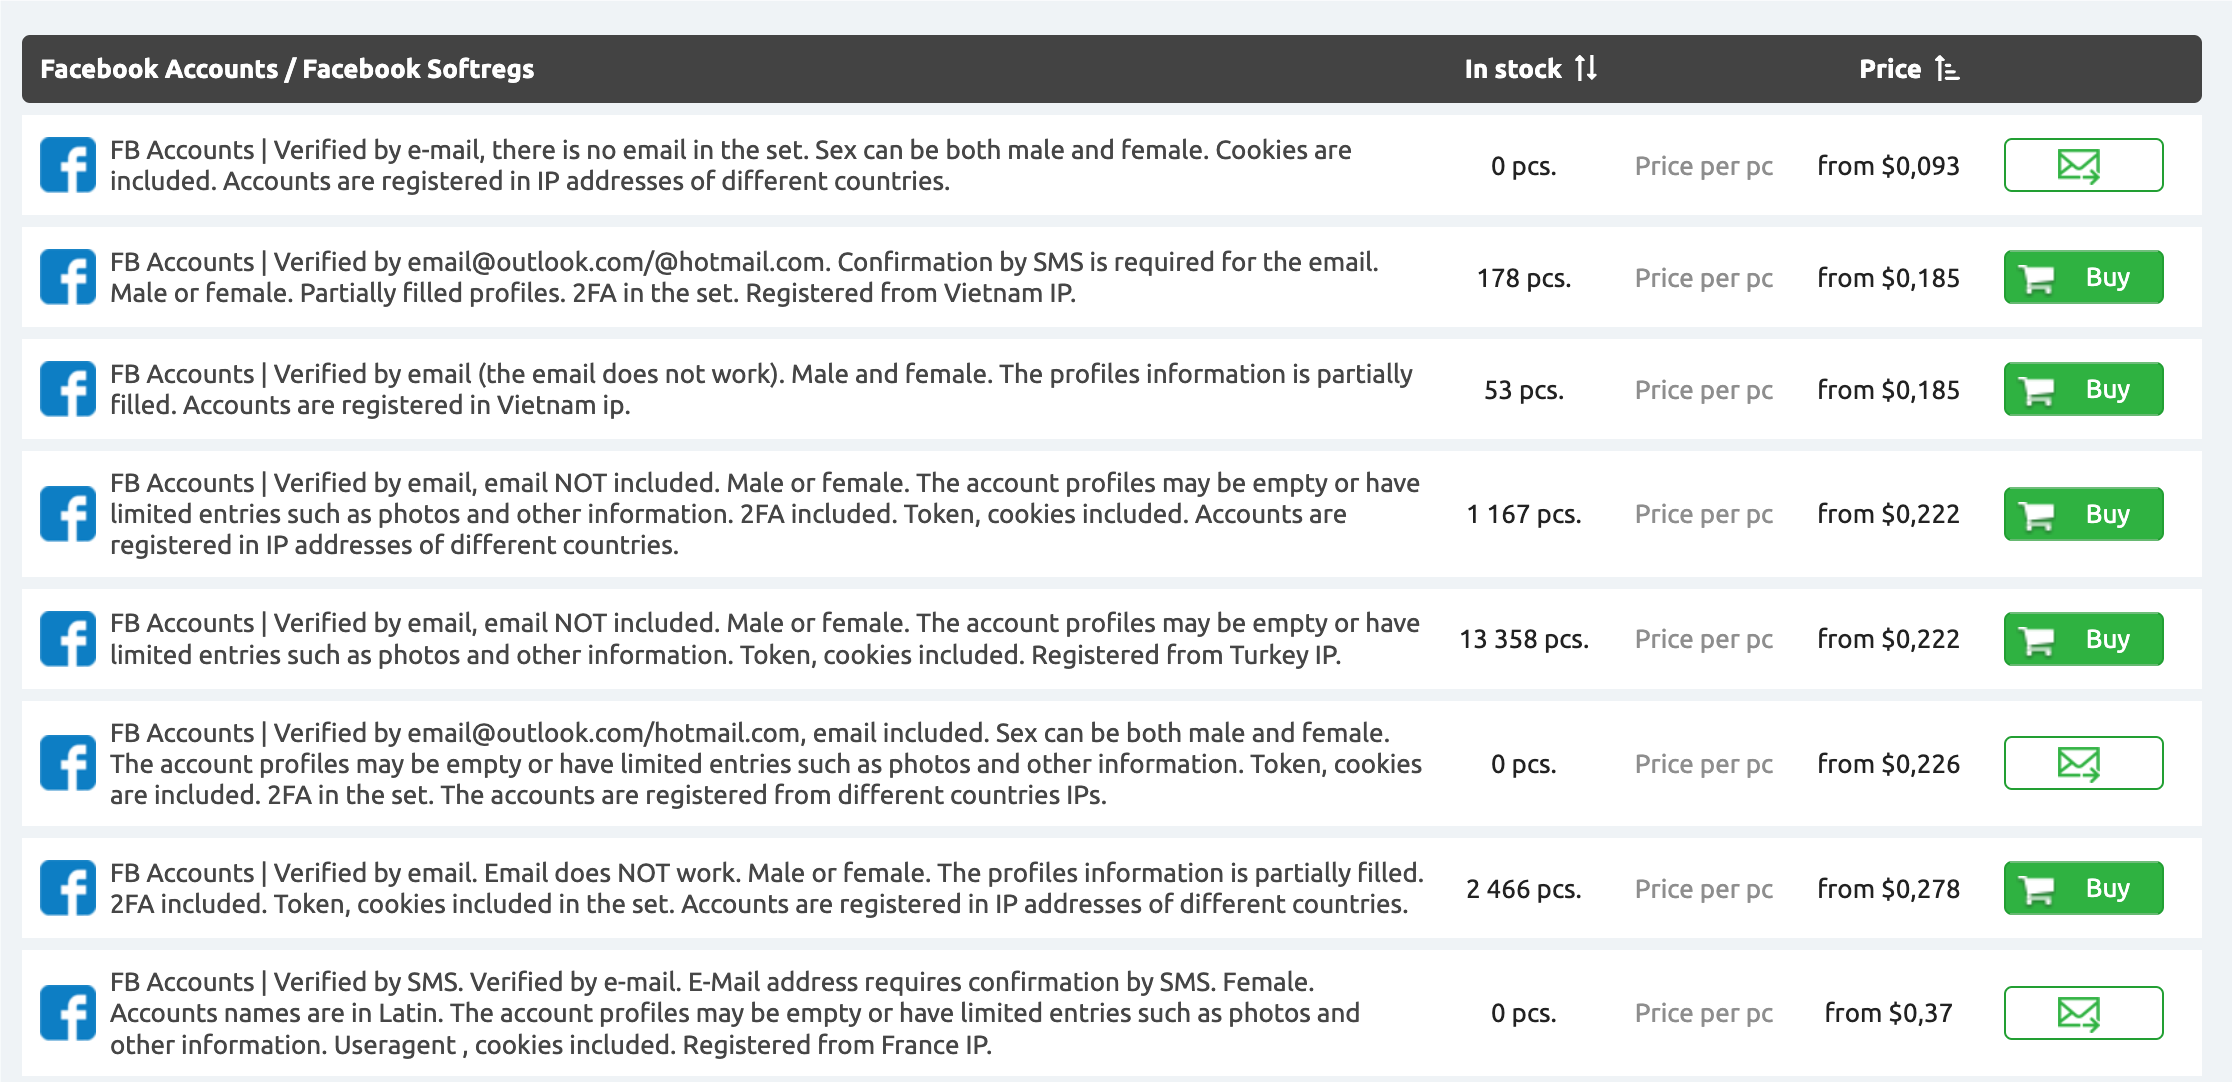
\includegraphics[scale=.1]{assets/accs1.png}\pause

		\vspace{-48pt}
		\noindent\hskip9em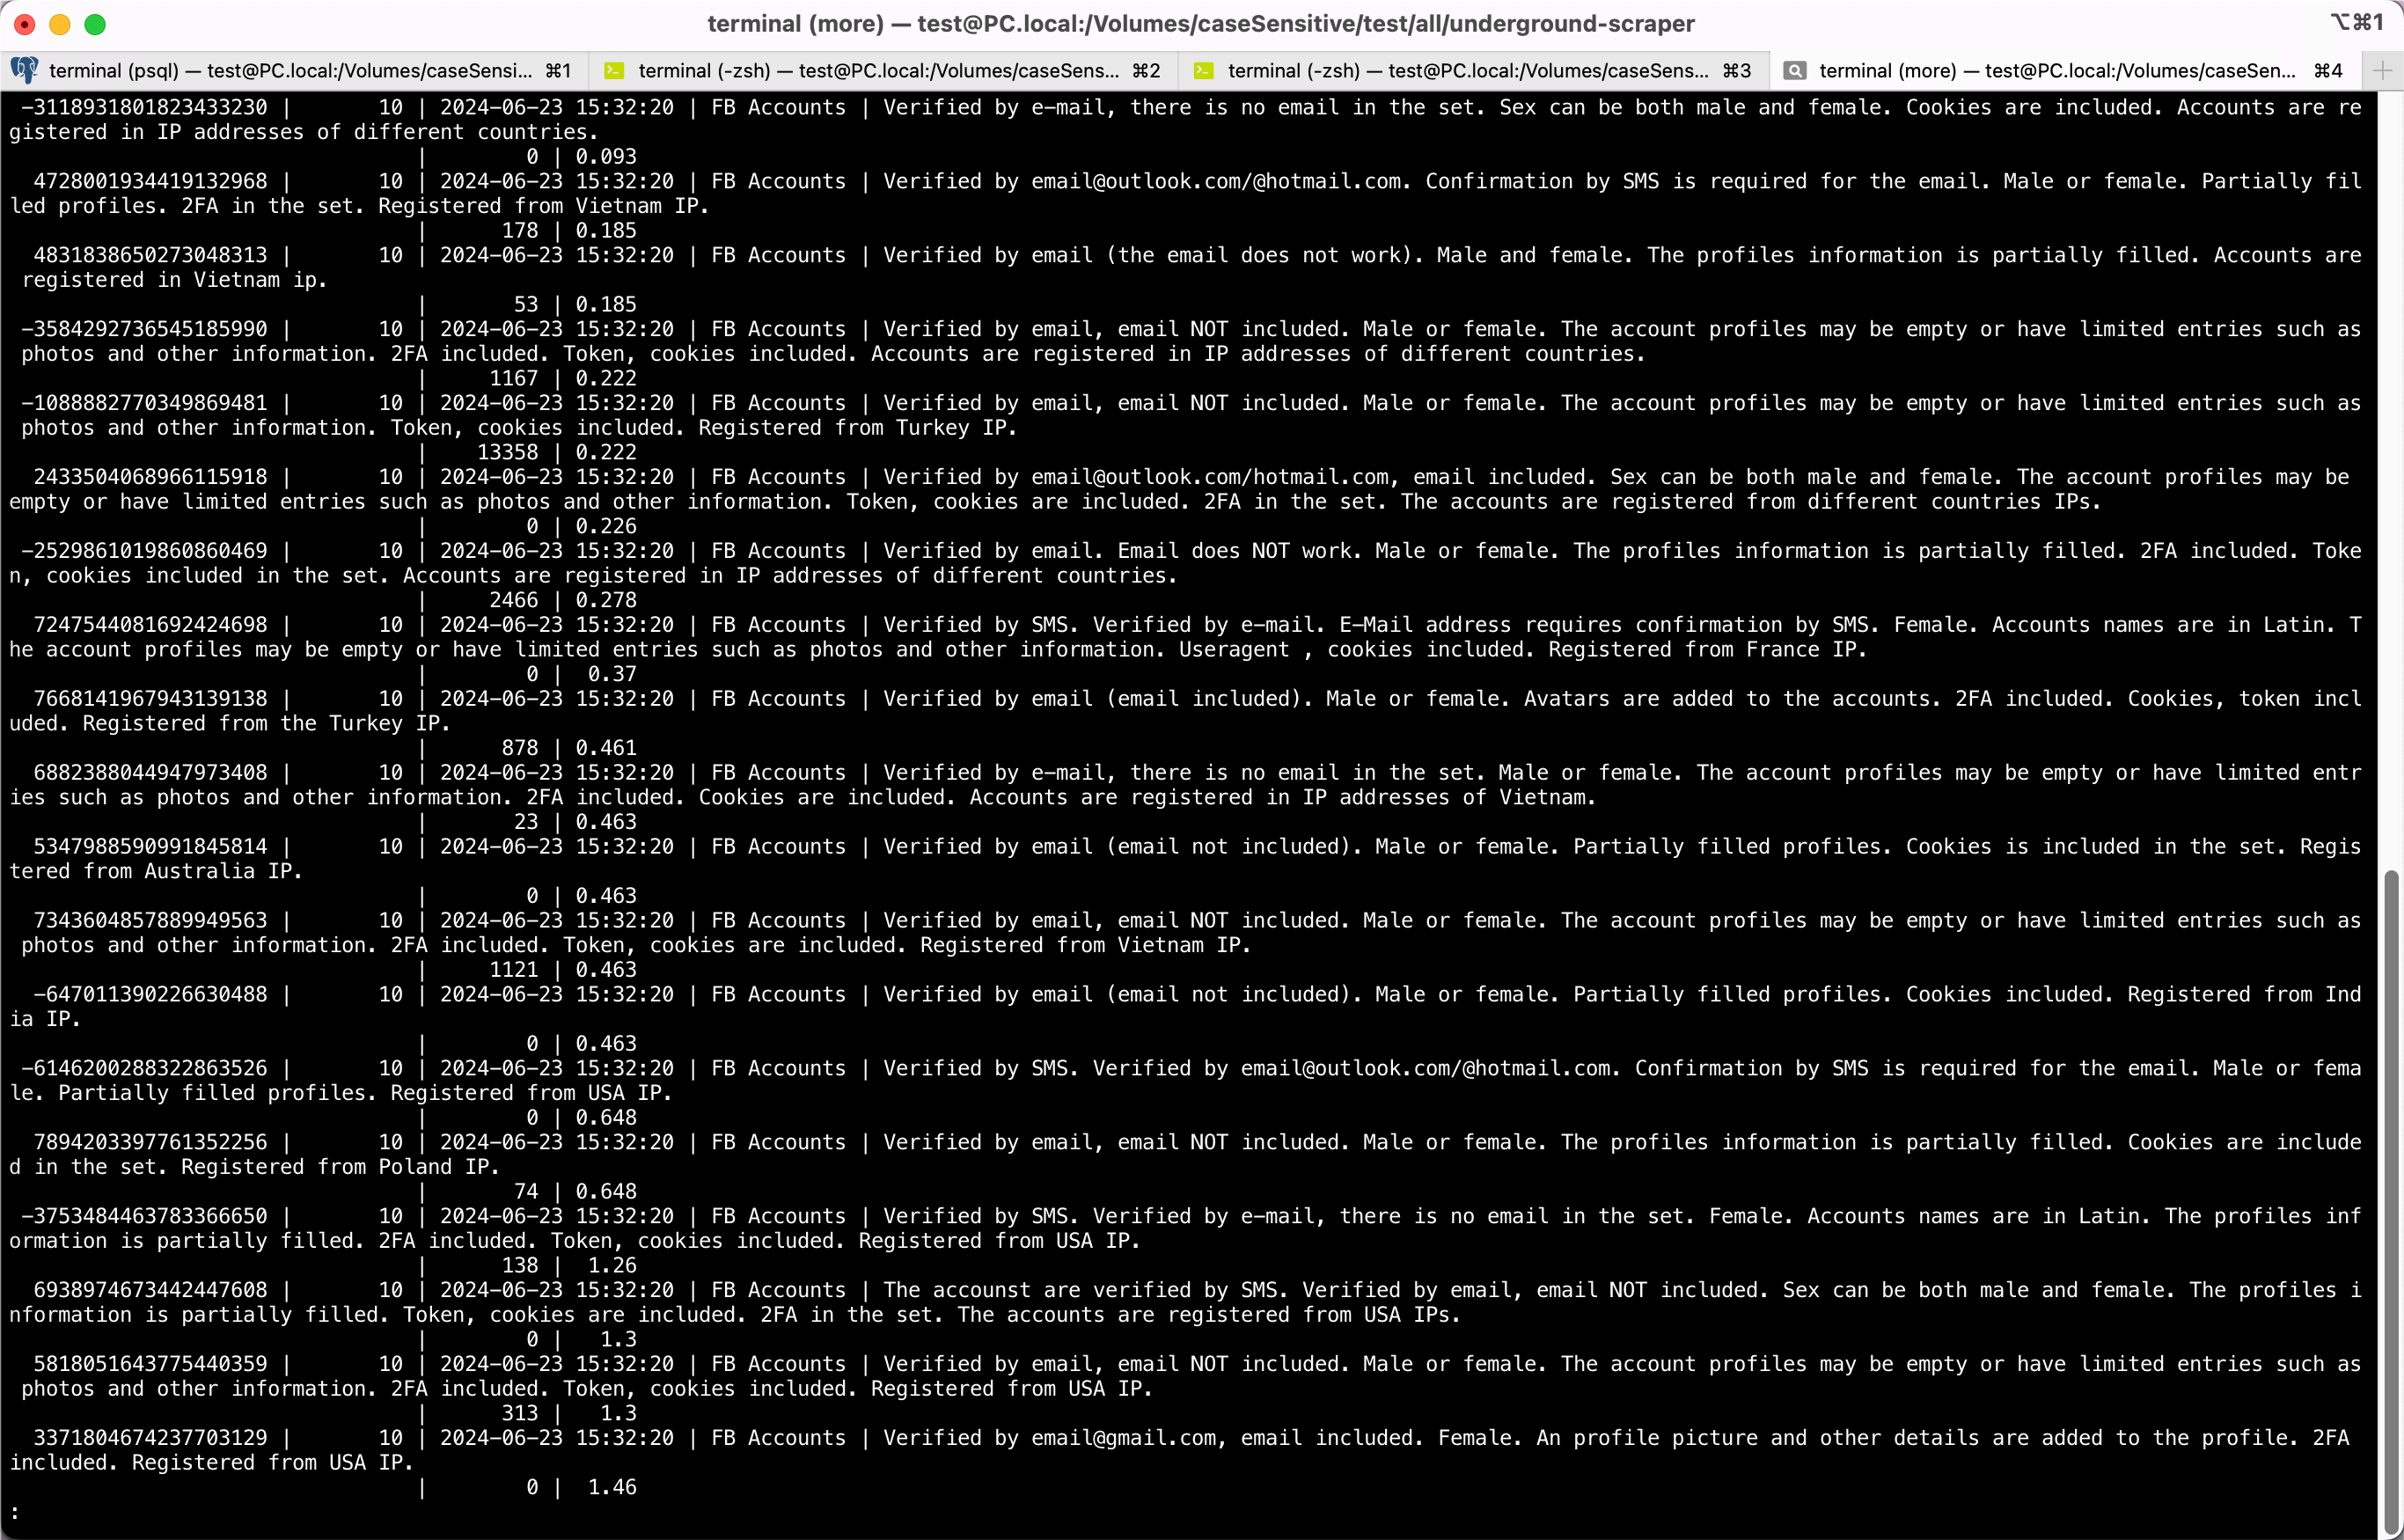
\includegraphics[scale=.08]{assets/accs2.png}
	}

	\frame {
		\begin{figure}
			\centering
			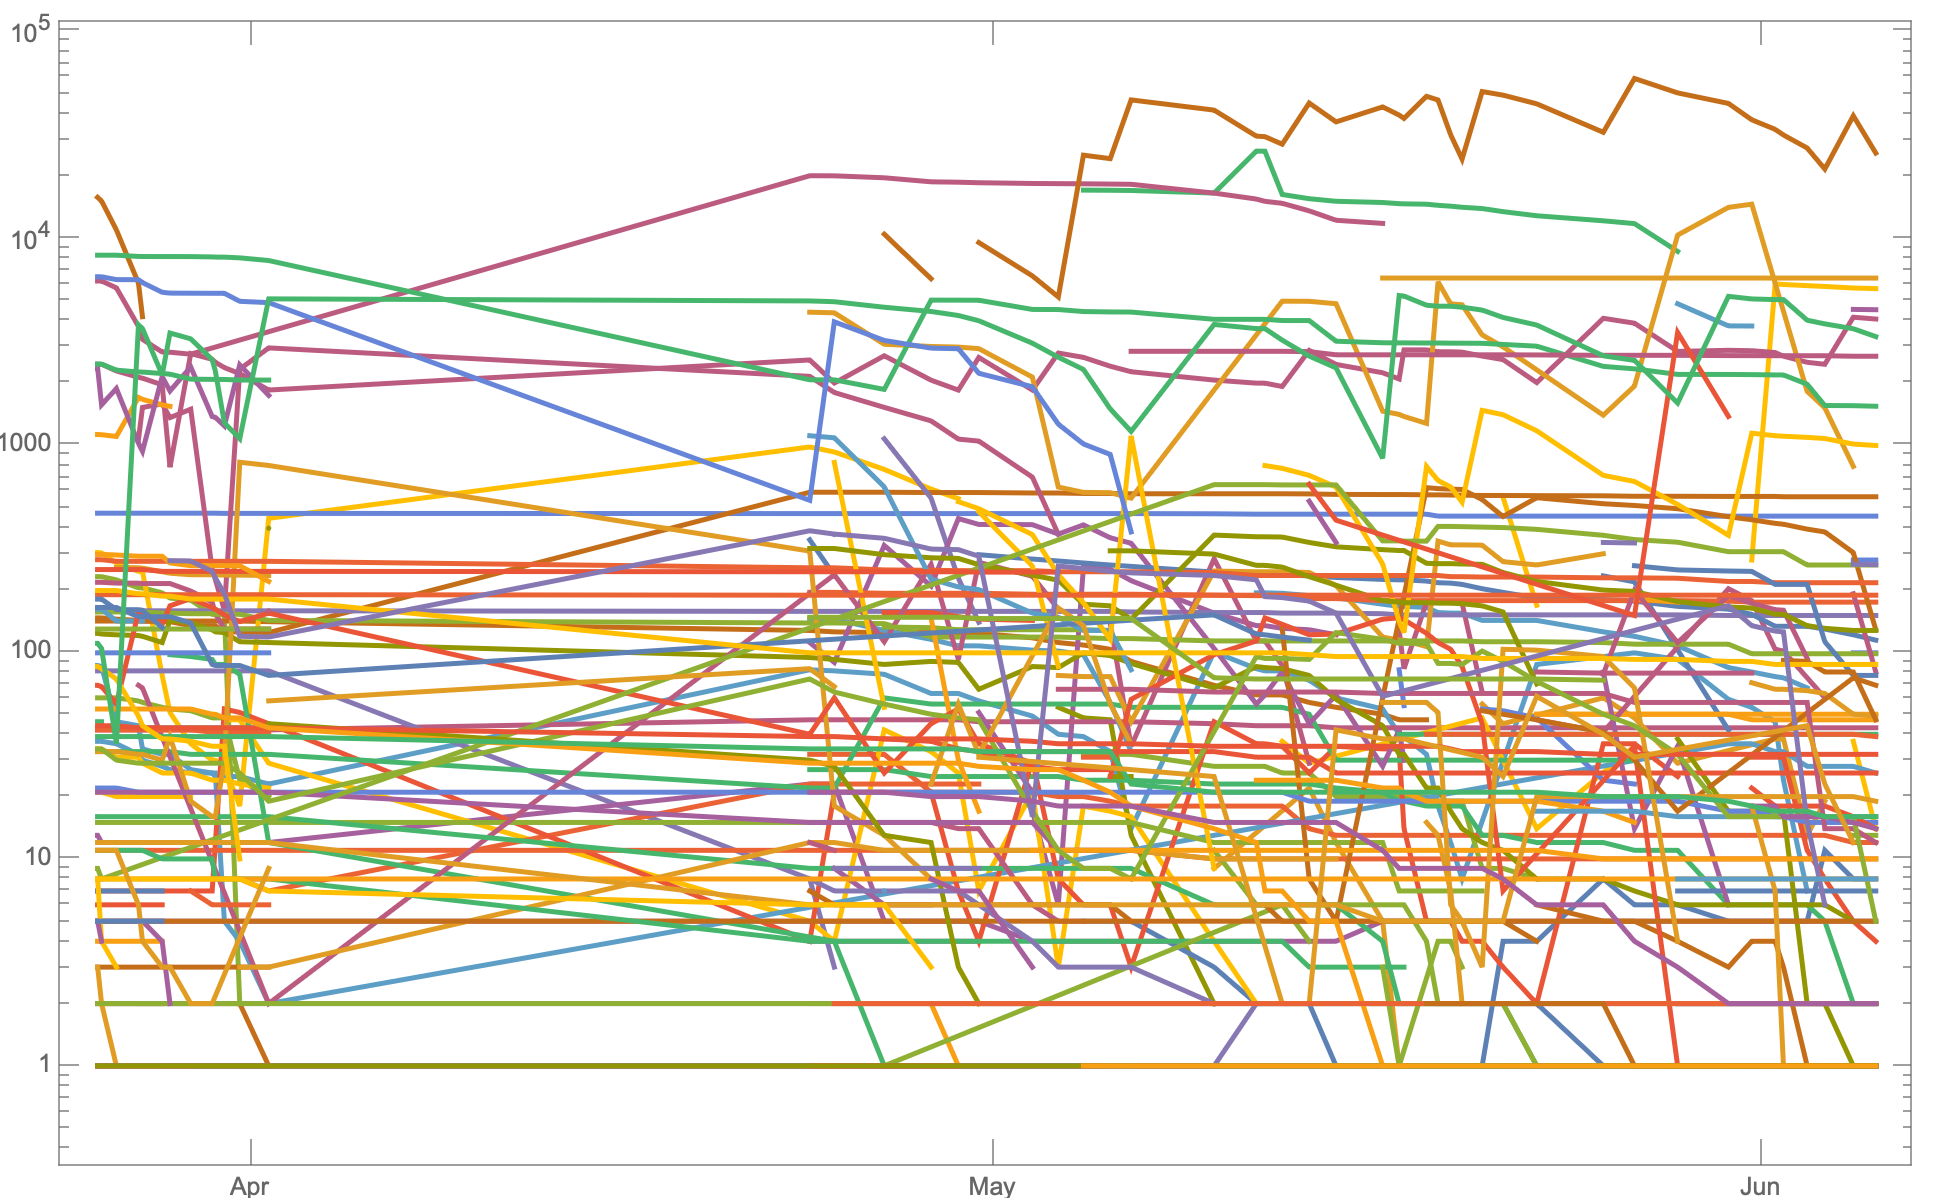
\includegraphics[scale=.15]{assets/accs3.png}
			\caption{Quantity--time curve}
		\end{figure}
	}

	\subsubsection{EZKIFY Serivces}

	\frame {
		\noindent\hskip-1.5em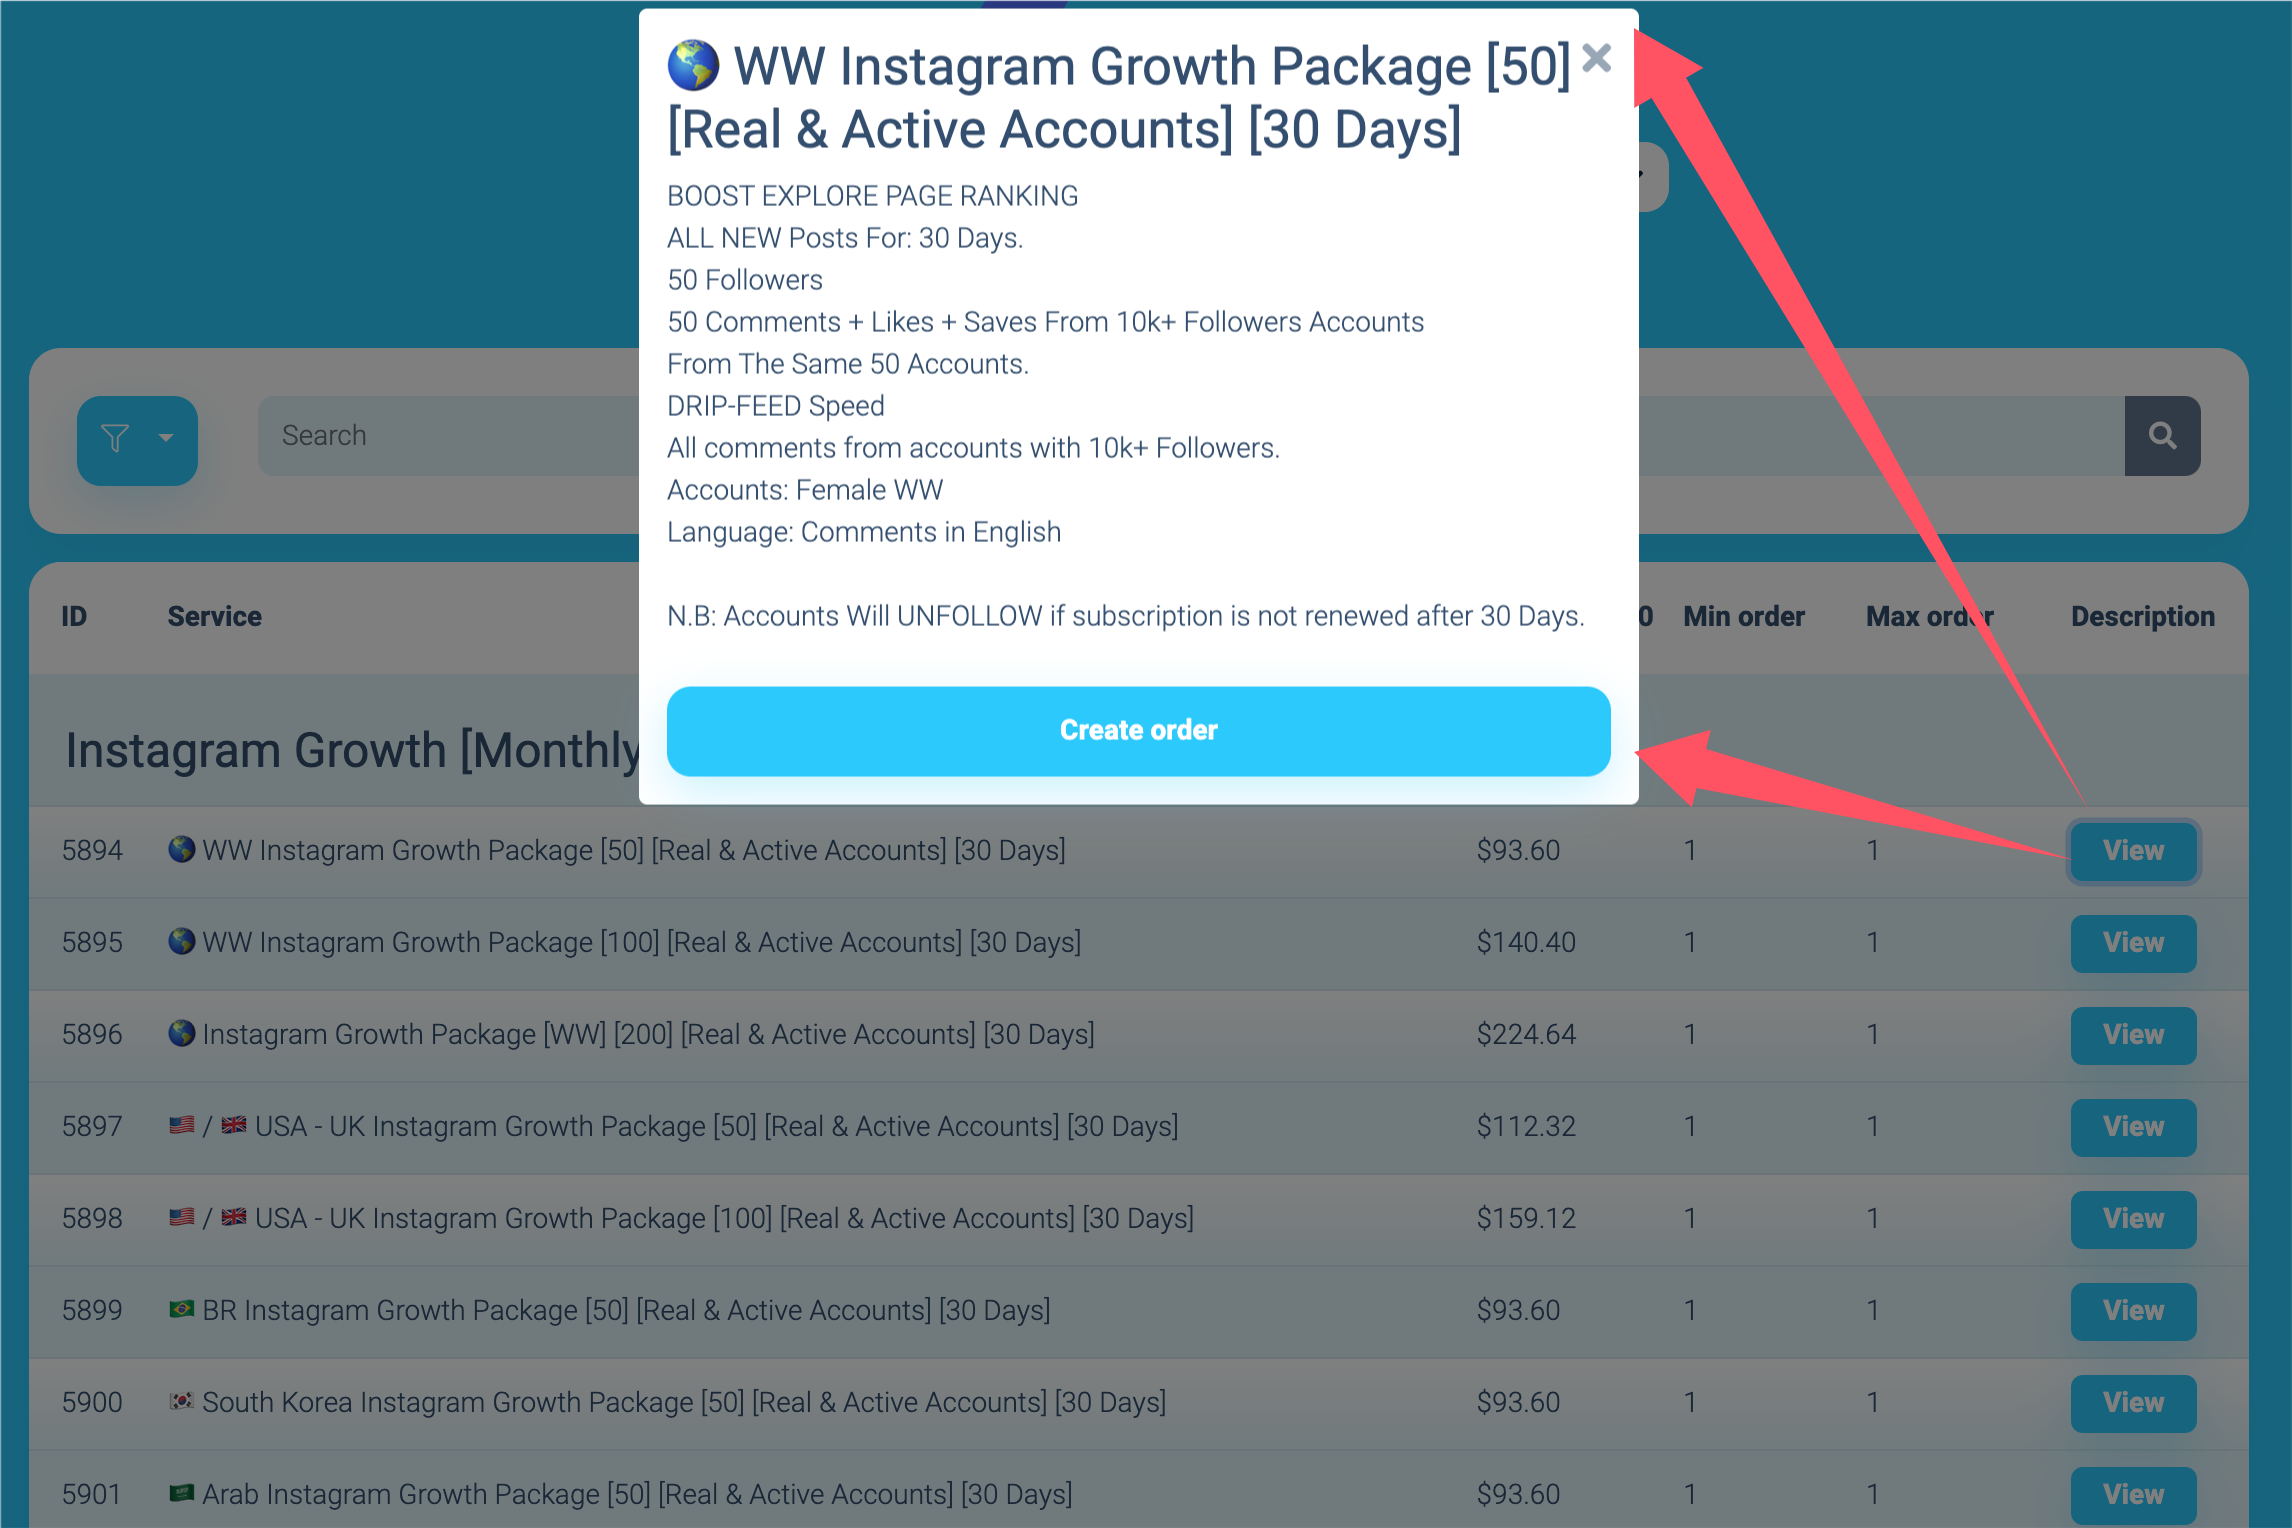
\includegraphics[scale=.09]{assets/ez1.png}\pause

		\vspace{-58pt}
		\noindent\hskip11.7em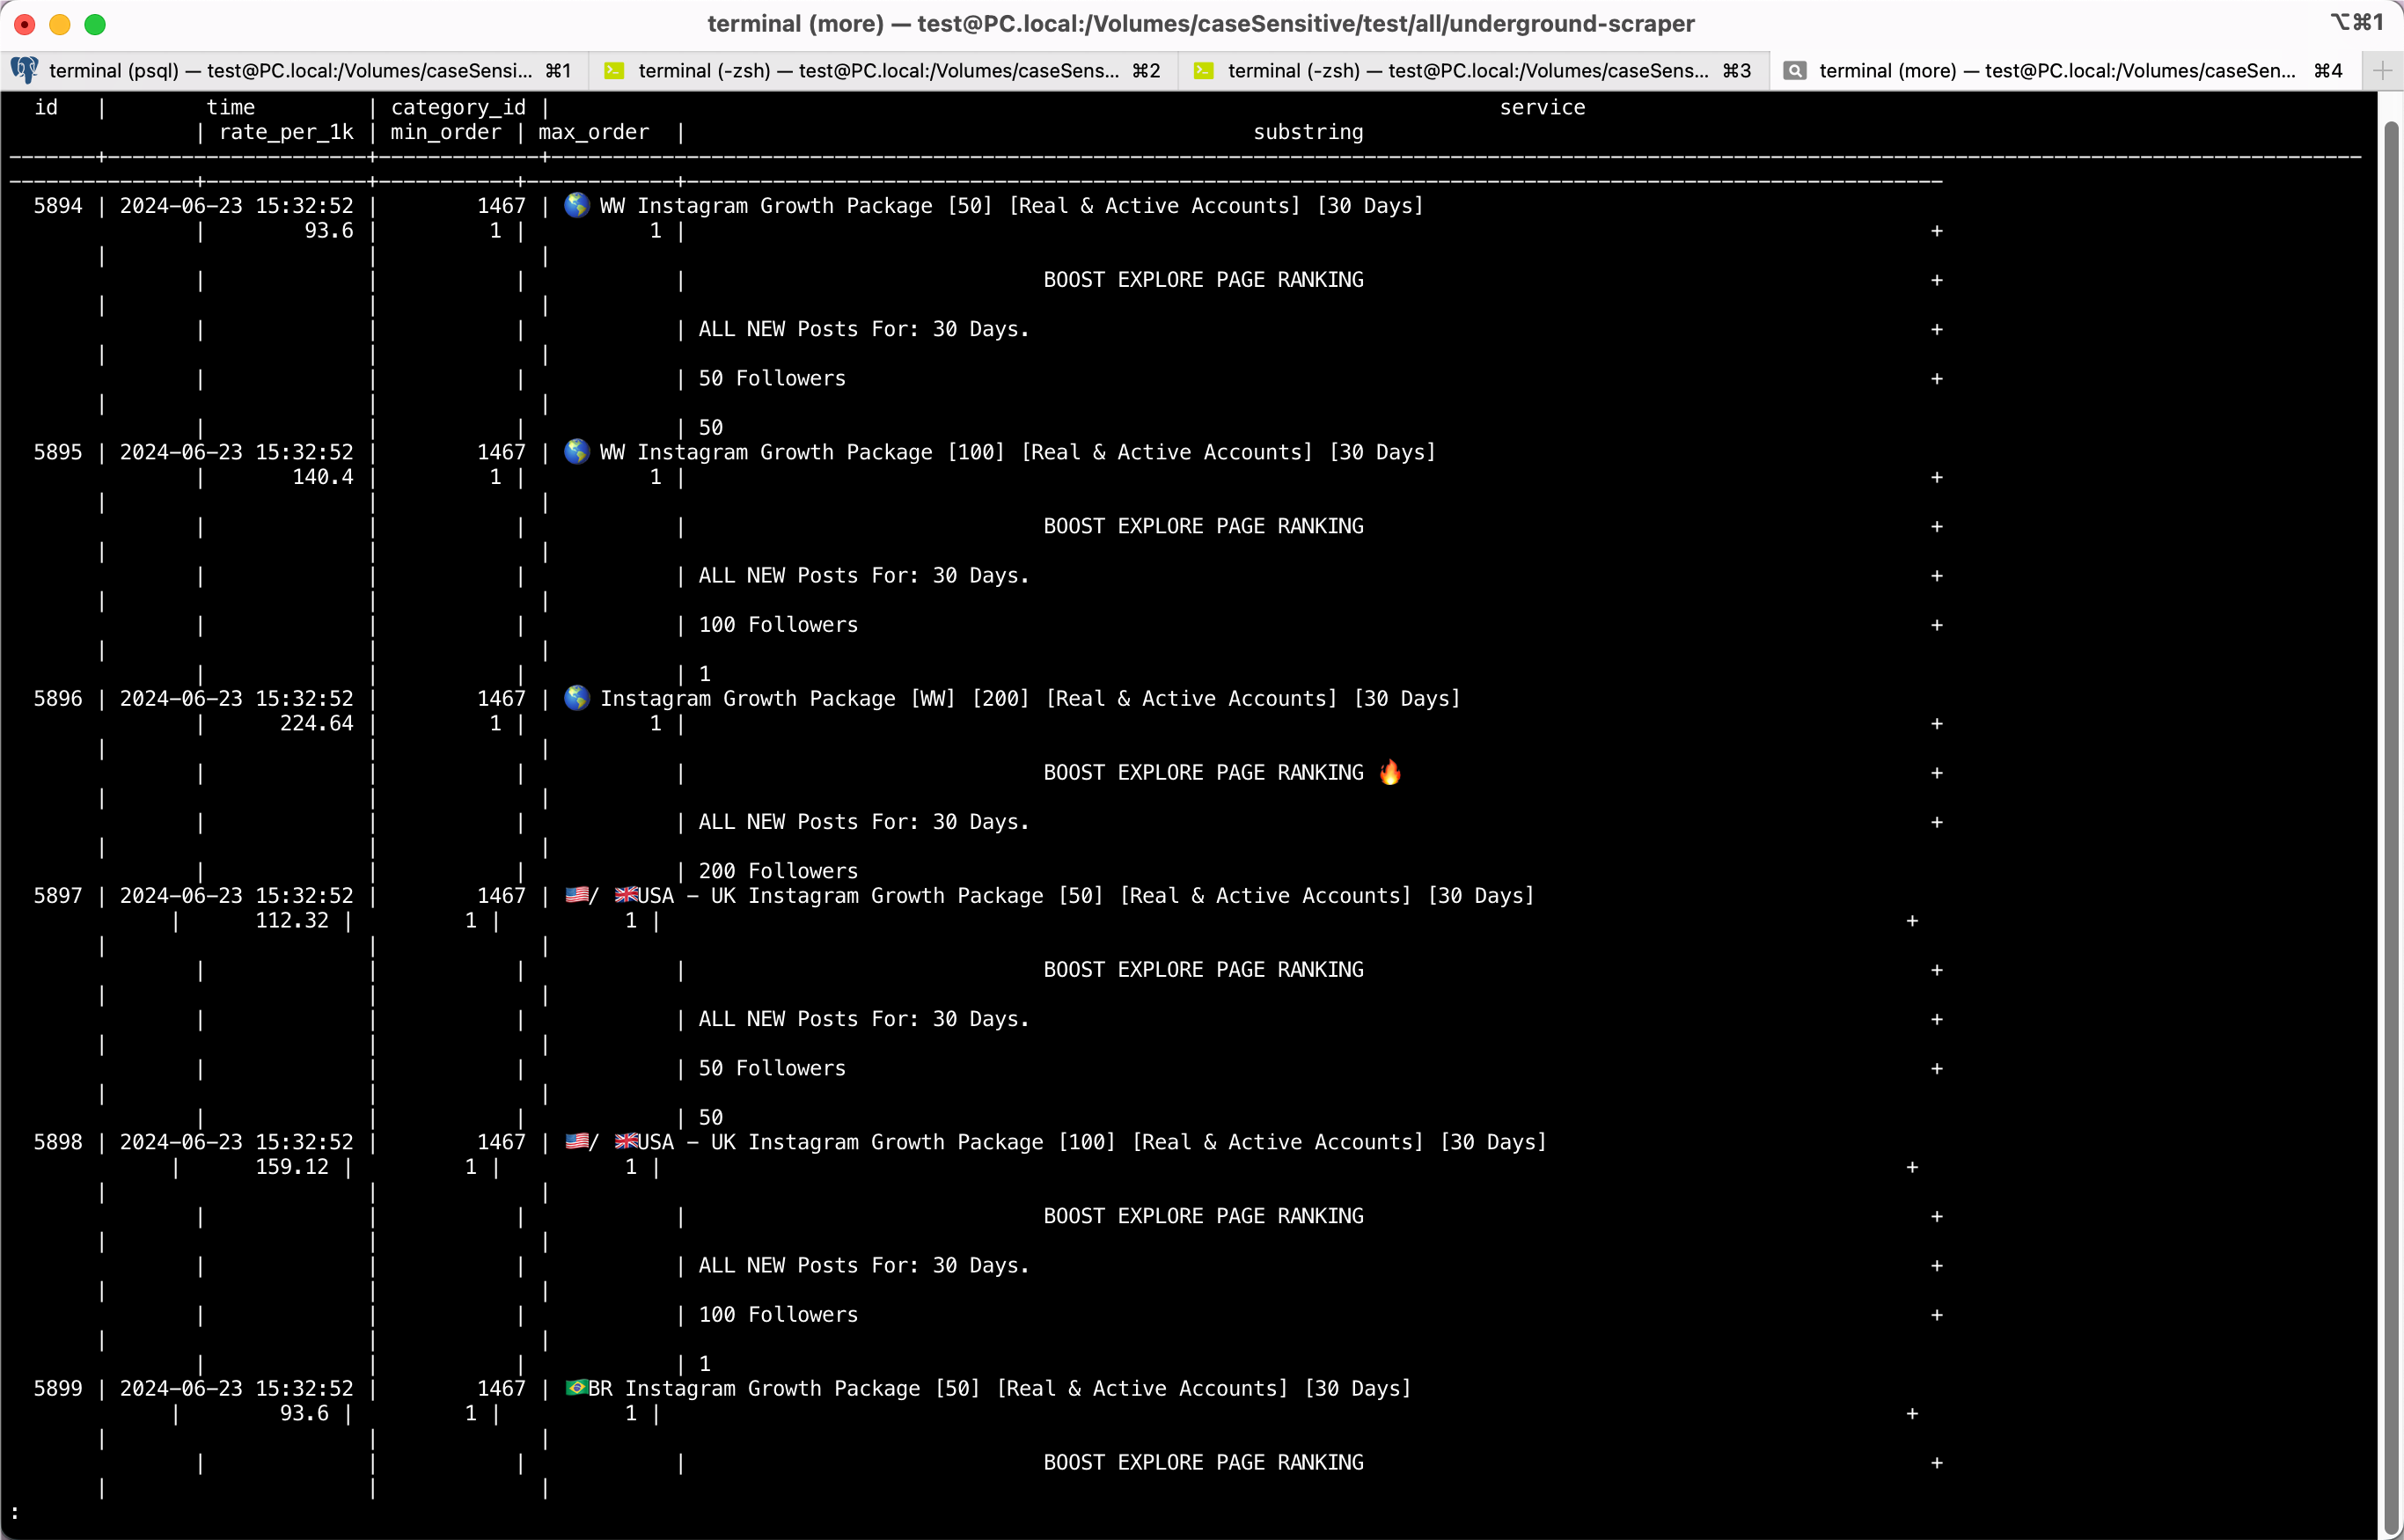
\includegraphics[scale=.075]{assets/ez2.png}
	}

	\subsubsection{BlackHatWorld}

	\frame {
		\centering
		\alt<2>{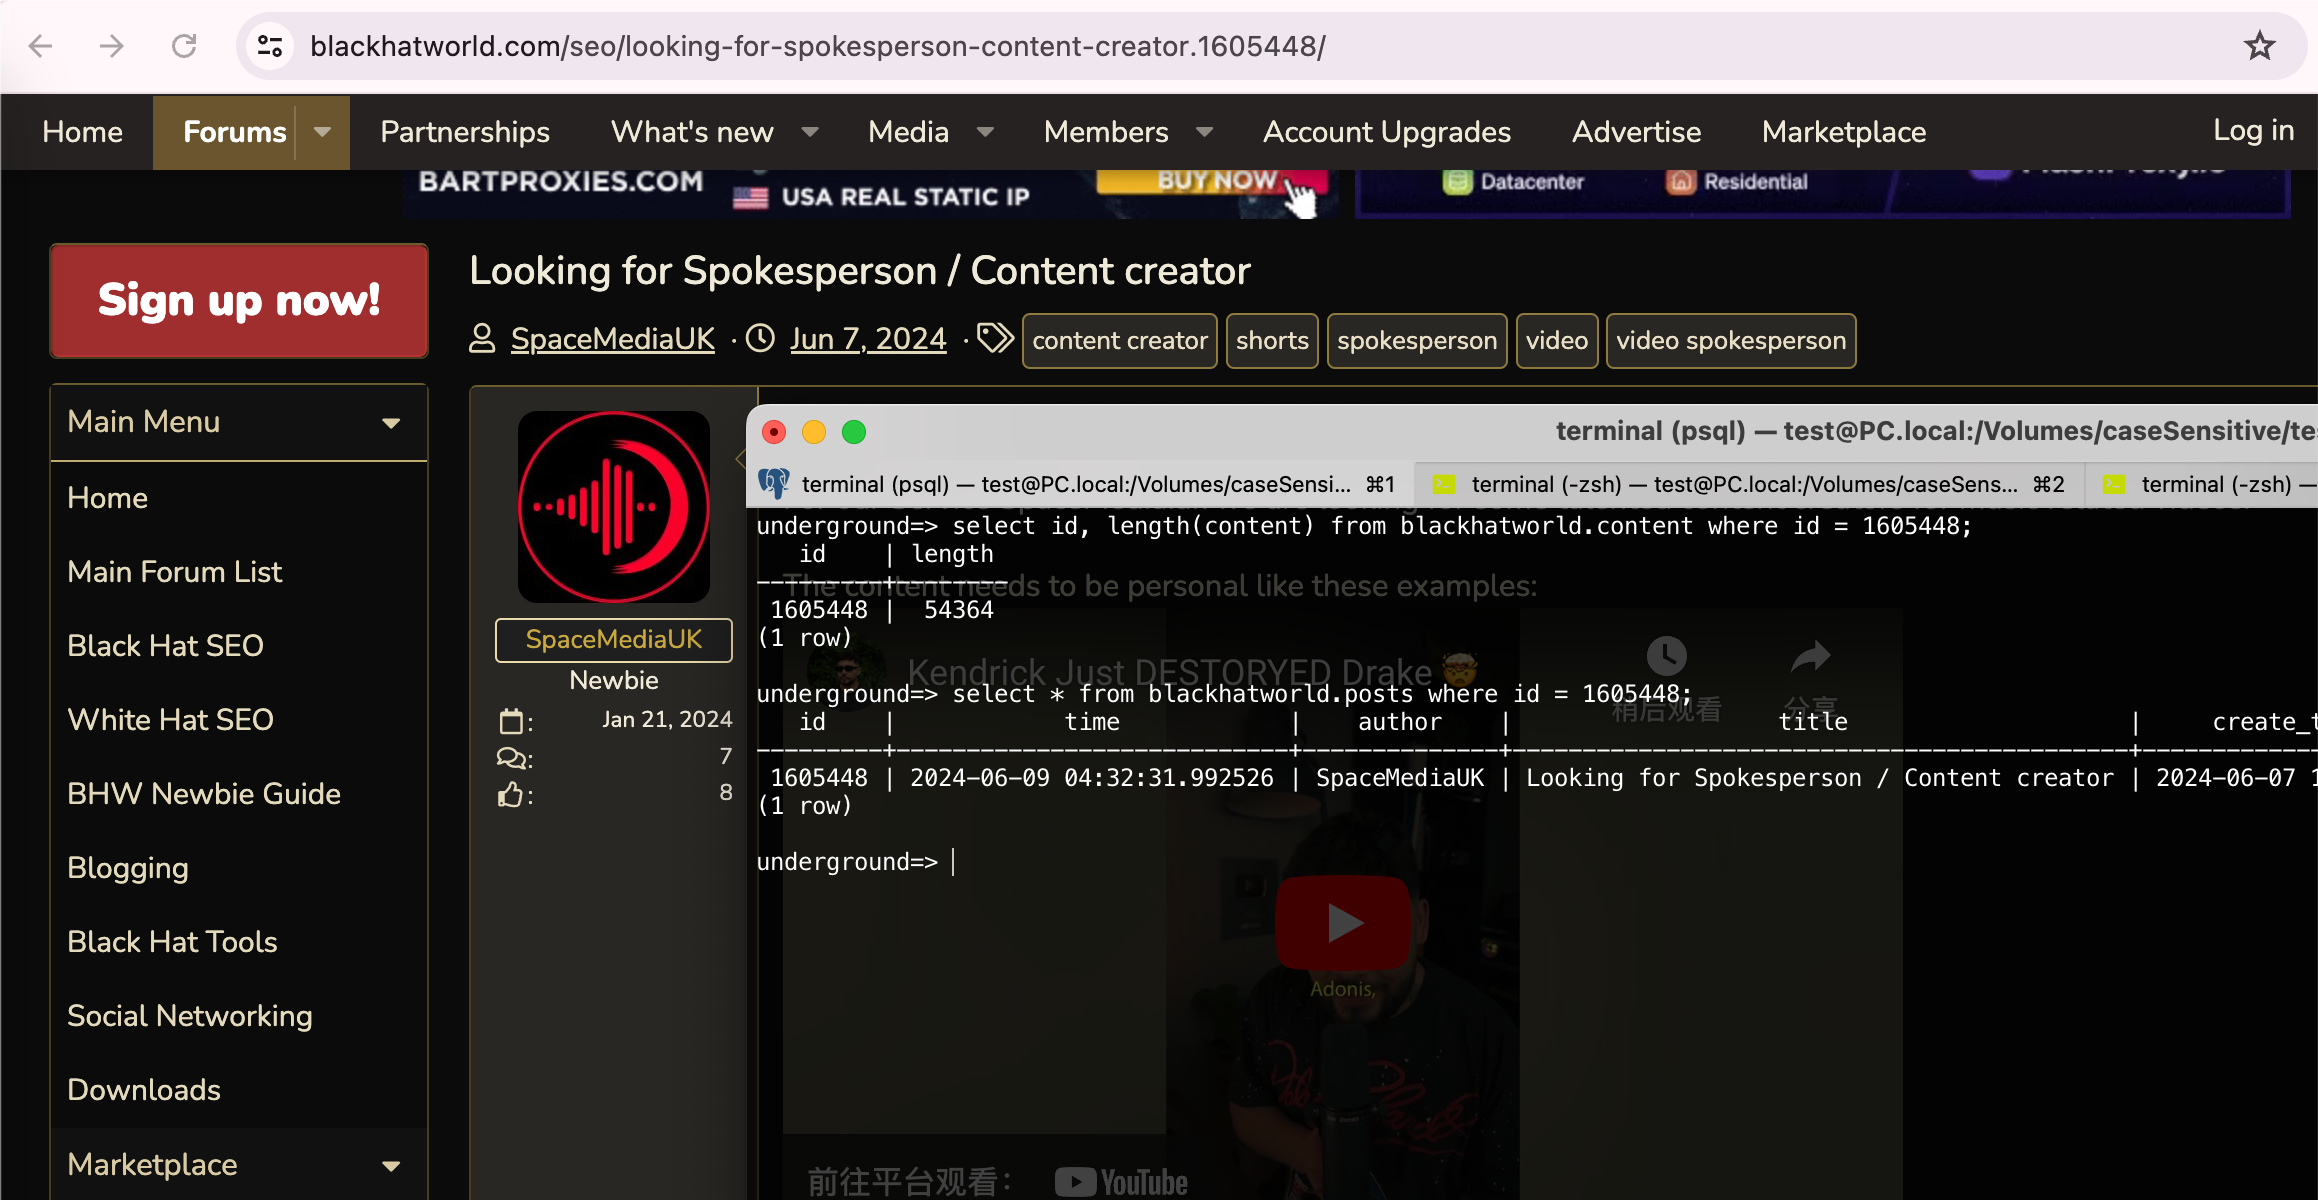
\includegraphics[scale=.14]{assets/bhw2.png}}{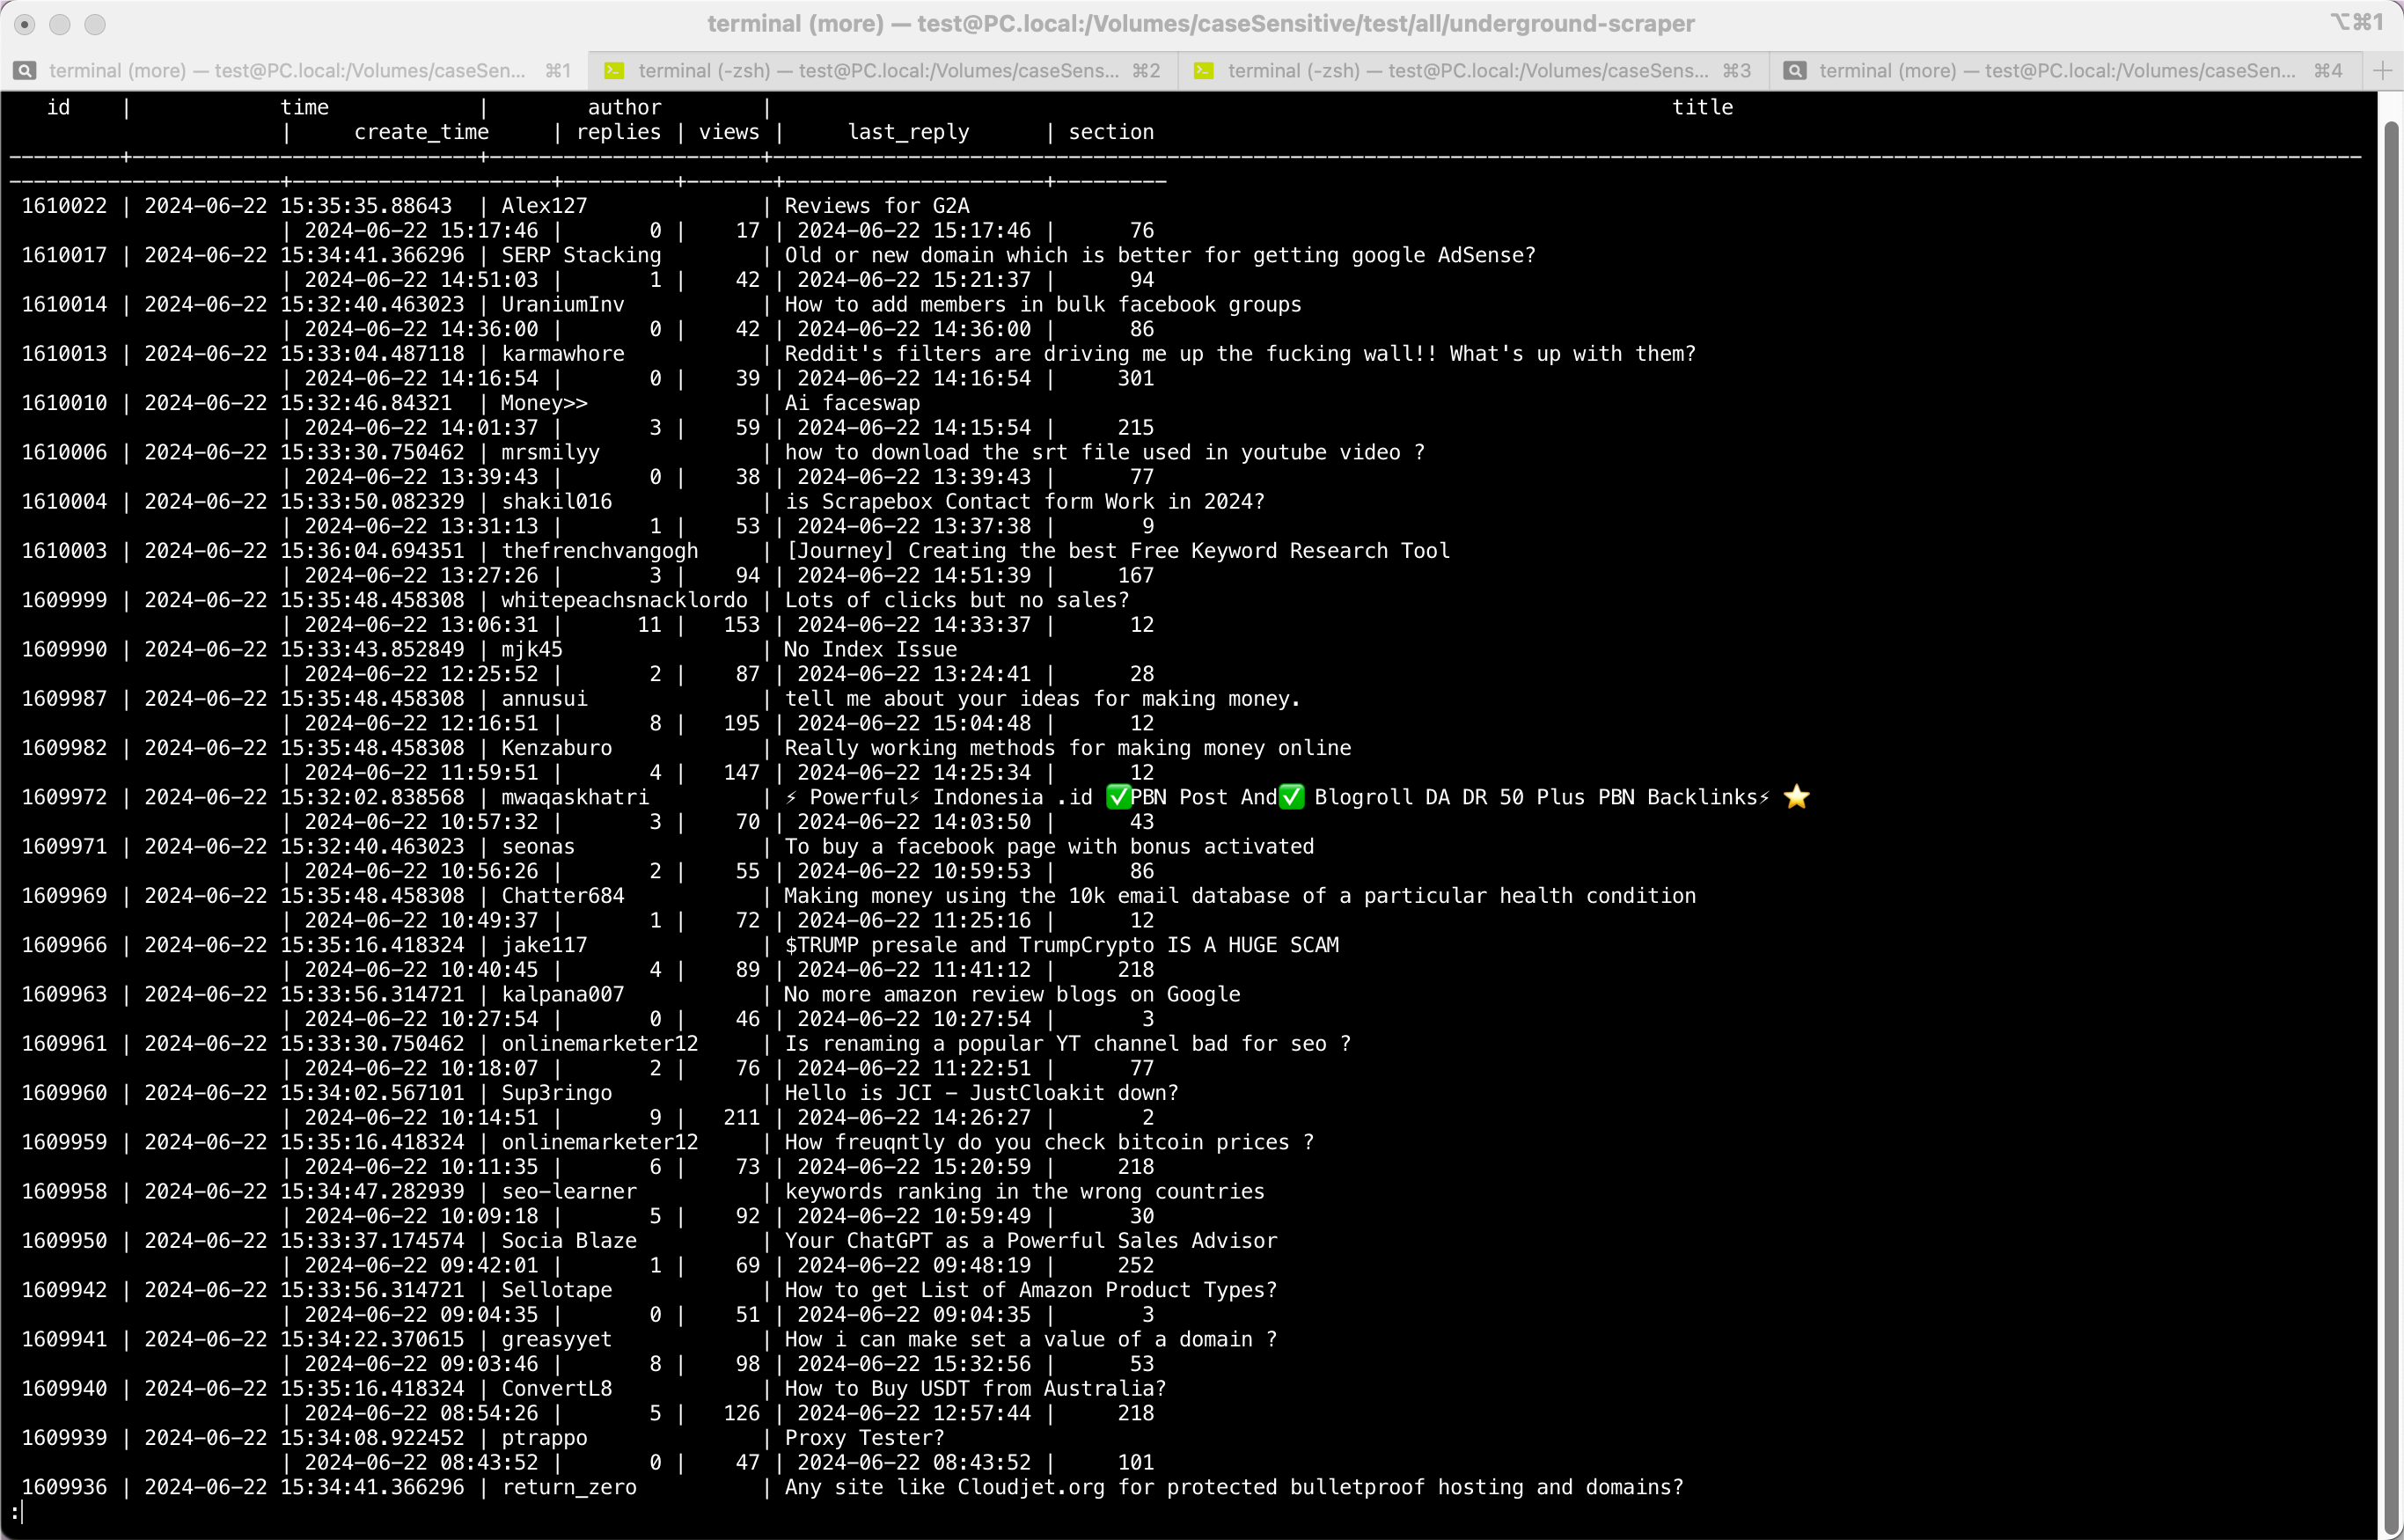
\includegraphics[scale=.11]{assets/bhw1.png}}
	}
\fi
	\section[UGM\,scraper]{Underground market scraper}

	\frame {%
		\begin{columns}[c]%
			\begin{column}[c]{321pt}%
				\begin{multicols}2%
					\tableofcontents[currentsection,subsubsectionstyle=hide]%
				\end{multicols}%
			\end{column}%
		\end{columns}%
	}
\iftrue
	\subsection{Overview}

	\frame {
		\noindent
		\begin{minipage}{0.24\linewidth}
			\noindent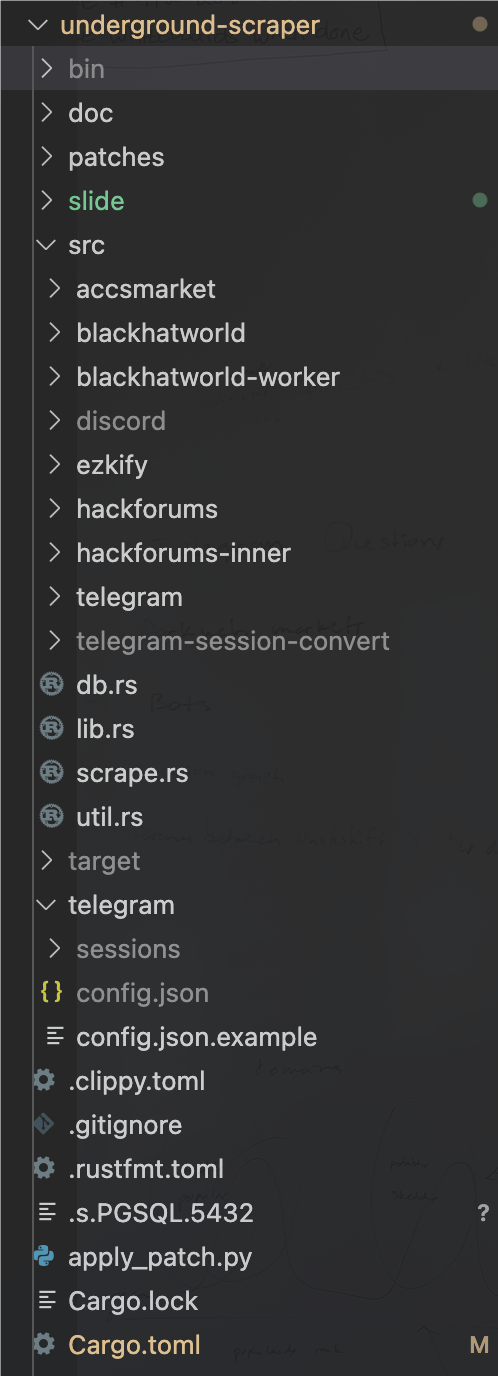
\includegraphics[scale=.15]{assets/structure.png}
		\end{minipage}\pause
		\begin{minipage}{0.75\linewidth}
			\begin{itemize}
				\item Written in 
\includegraphics[scale=.03]{assets/ferris.png}Rust\pause
					\begin{itemize}
						\item \uwave{Efficient} in computing (e.g., string parsing)\pause
						\item \uwave{Friendly} async/multi-threading\pause
						\item \uwave{Robust} error handling, stable and uninterrupted background tasks\pause
						\item \uwave{Strong maintainability}, durable to use
					\end{itemize}\pause
				\item Repo: \compress{-32pt}{\footnotesize https://github.com/yhx-12243/underground-scraper}\pause
					\begin{itemize}
						\item Detailed and comprehensive README file\pause
						\item Currently not public, may port to our group/other Git platform
					\end{itemize}
			\end{itemize}
		\end{minipage}
	}

	\subsection{General Usage}

	\subsubsection{Prerequisites}

	\begin{frame}[fragile]
		\begin{enumerate}
			\item Requirements:\pause
				\begin{itemize}
					\item A 
\includegraphics[scale=.03]{assets/ferris.png}Rust toolchain in a \texttt{nightly} version\pause
					\item 
\includegraphics[scale=.016]{assets/postgres.png}PostgreSQL environment, used as main data storage\pause
					\item 
\includegraphics[scale=.035]{assets/chromedriver.png}ChromeDriver, used to solve Cloudflare CAPTCHA
				\end{itemize}\pause
			\item Patches:\pause
				\begin{itemize}
					\item Simply, just run \texttt{./apply\char95patch.py}\pause
					\item Thoughtful. Reentrant.
				\end{itemize}\pause
			\item Environment variables:\pause
				\footnotesize\begin{minted}[frame=single,linenos=true,rulecolor=blue]{shell}
export DB_HOST=/var/run/postgresql
export DB_USER=postgres
export DB_NAME=postgres
export DB_PASSWORD=<password> # optional
export RUST_LOG=info
				\end{minted}
		\end{enumerate}
	\end{frame}

	\subsubsection{Build}

	\frame {
		\begin{enumerate}
			\addtocounter{enumi}3
			\item Building:\pause
				\begin{itemize}
					\item \texttt{cargo build -r}
				\end{itemize}\pause
			\item Running:\pause
				\begin{itemize}
					\item Binaries are in \texttt{./target/release/}\pause
					\item \texttt{cargo run -r --bin <name>} or copy them out
					\item For convenience, use \texttt{./foo <args>} denote \texttt{cargo run -r --bin foo -- <args>}
				\end{itemize}
		\end{enumerate}

	}

	\subsection{Specific Usage}

	\subsubsection{AccsMarket \& EZKIFY Services}

	\frame {
		Rationale:
		\begin{itemize}
			\item Use \texttt{reqwest} as inner client\pause
			\item Use \texttt{scraper} as parser
		\end{itemize}\pause

		Usage:
		\begin{itemize}
			\item Build PostgreSQL schema (see \texttt{README.md})\pause
			\item Just run \texttt{./accsmarket} and \texttt{./ezkify}\pause
			\item Add to \texttt{cron} jobs if possible
		\end{itemize}
	}

	\frame {
		\noindent\hskip-3.2em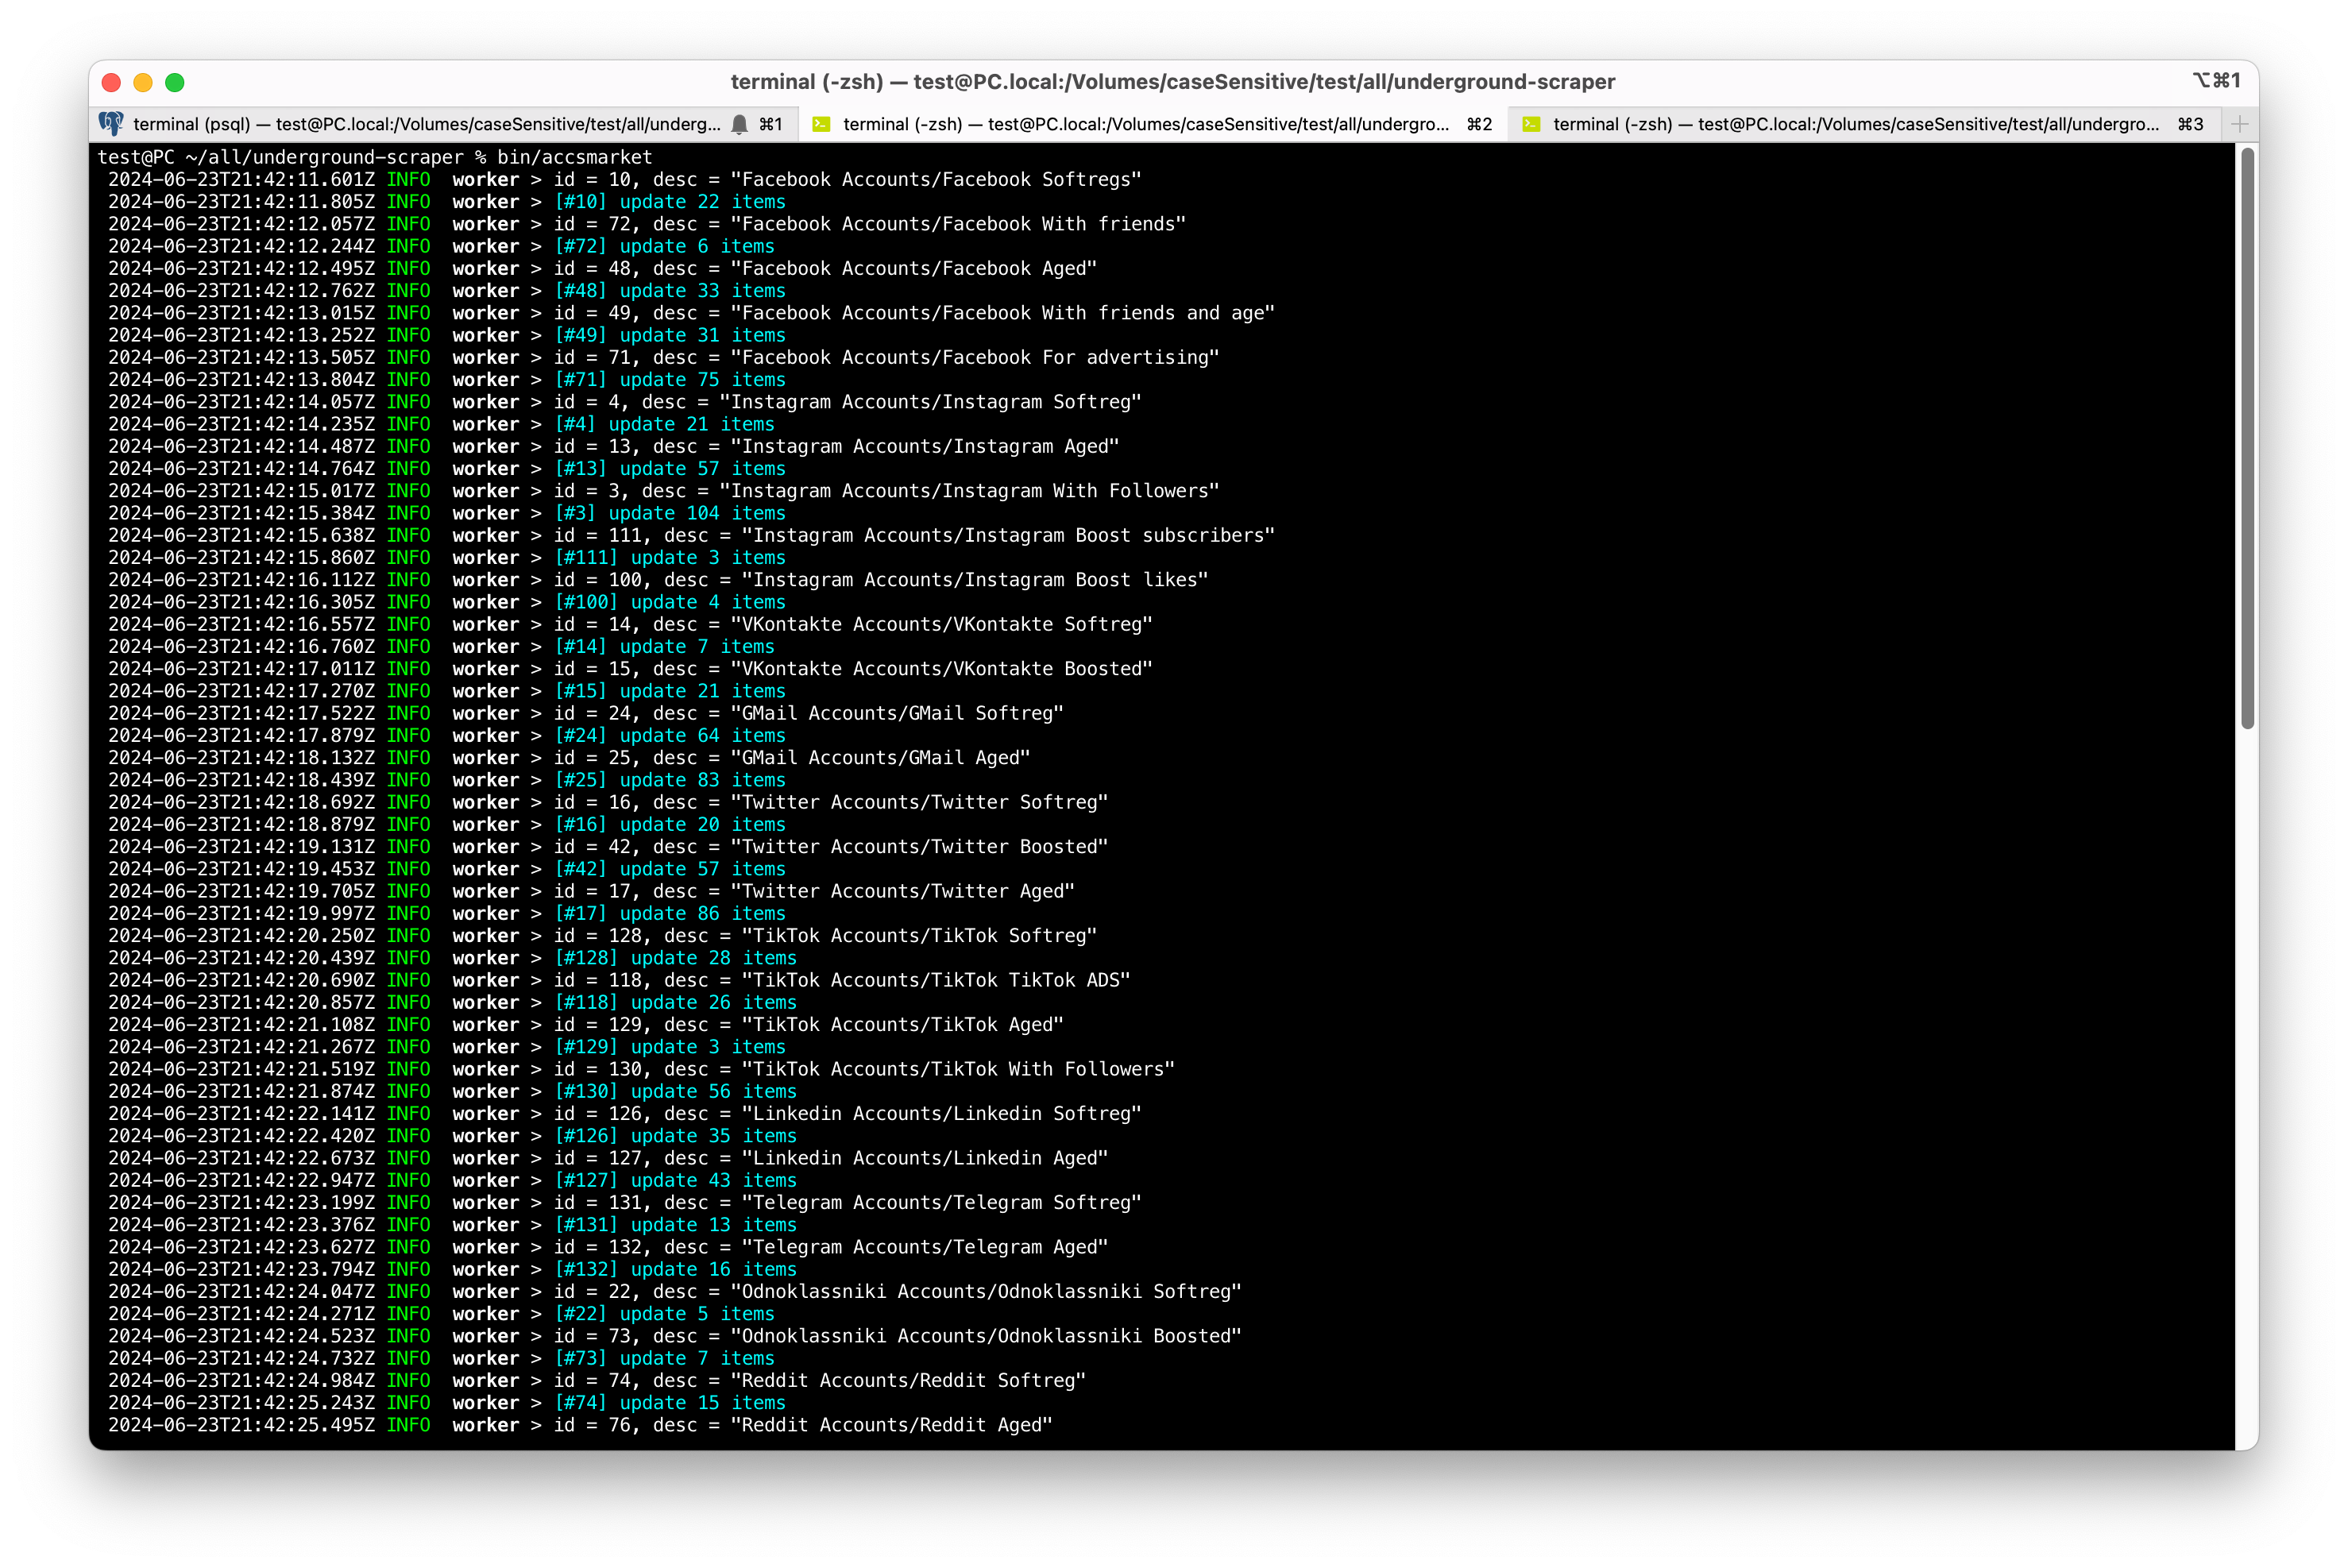
\includegraphics[scale=.17]{assets/c-a.png}

		\vspace{-108pt}
		\noindent\hskip8.3em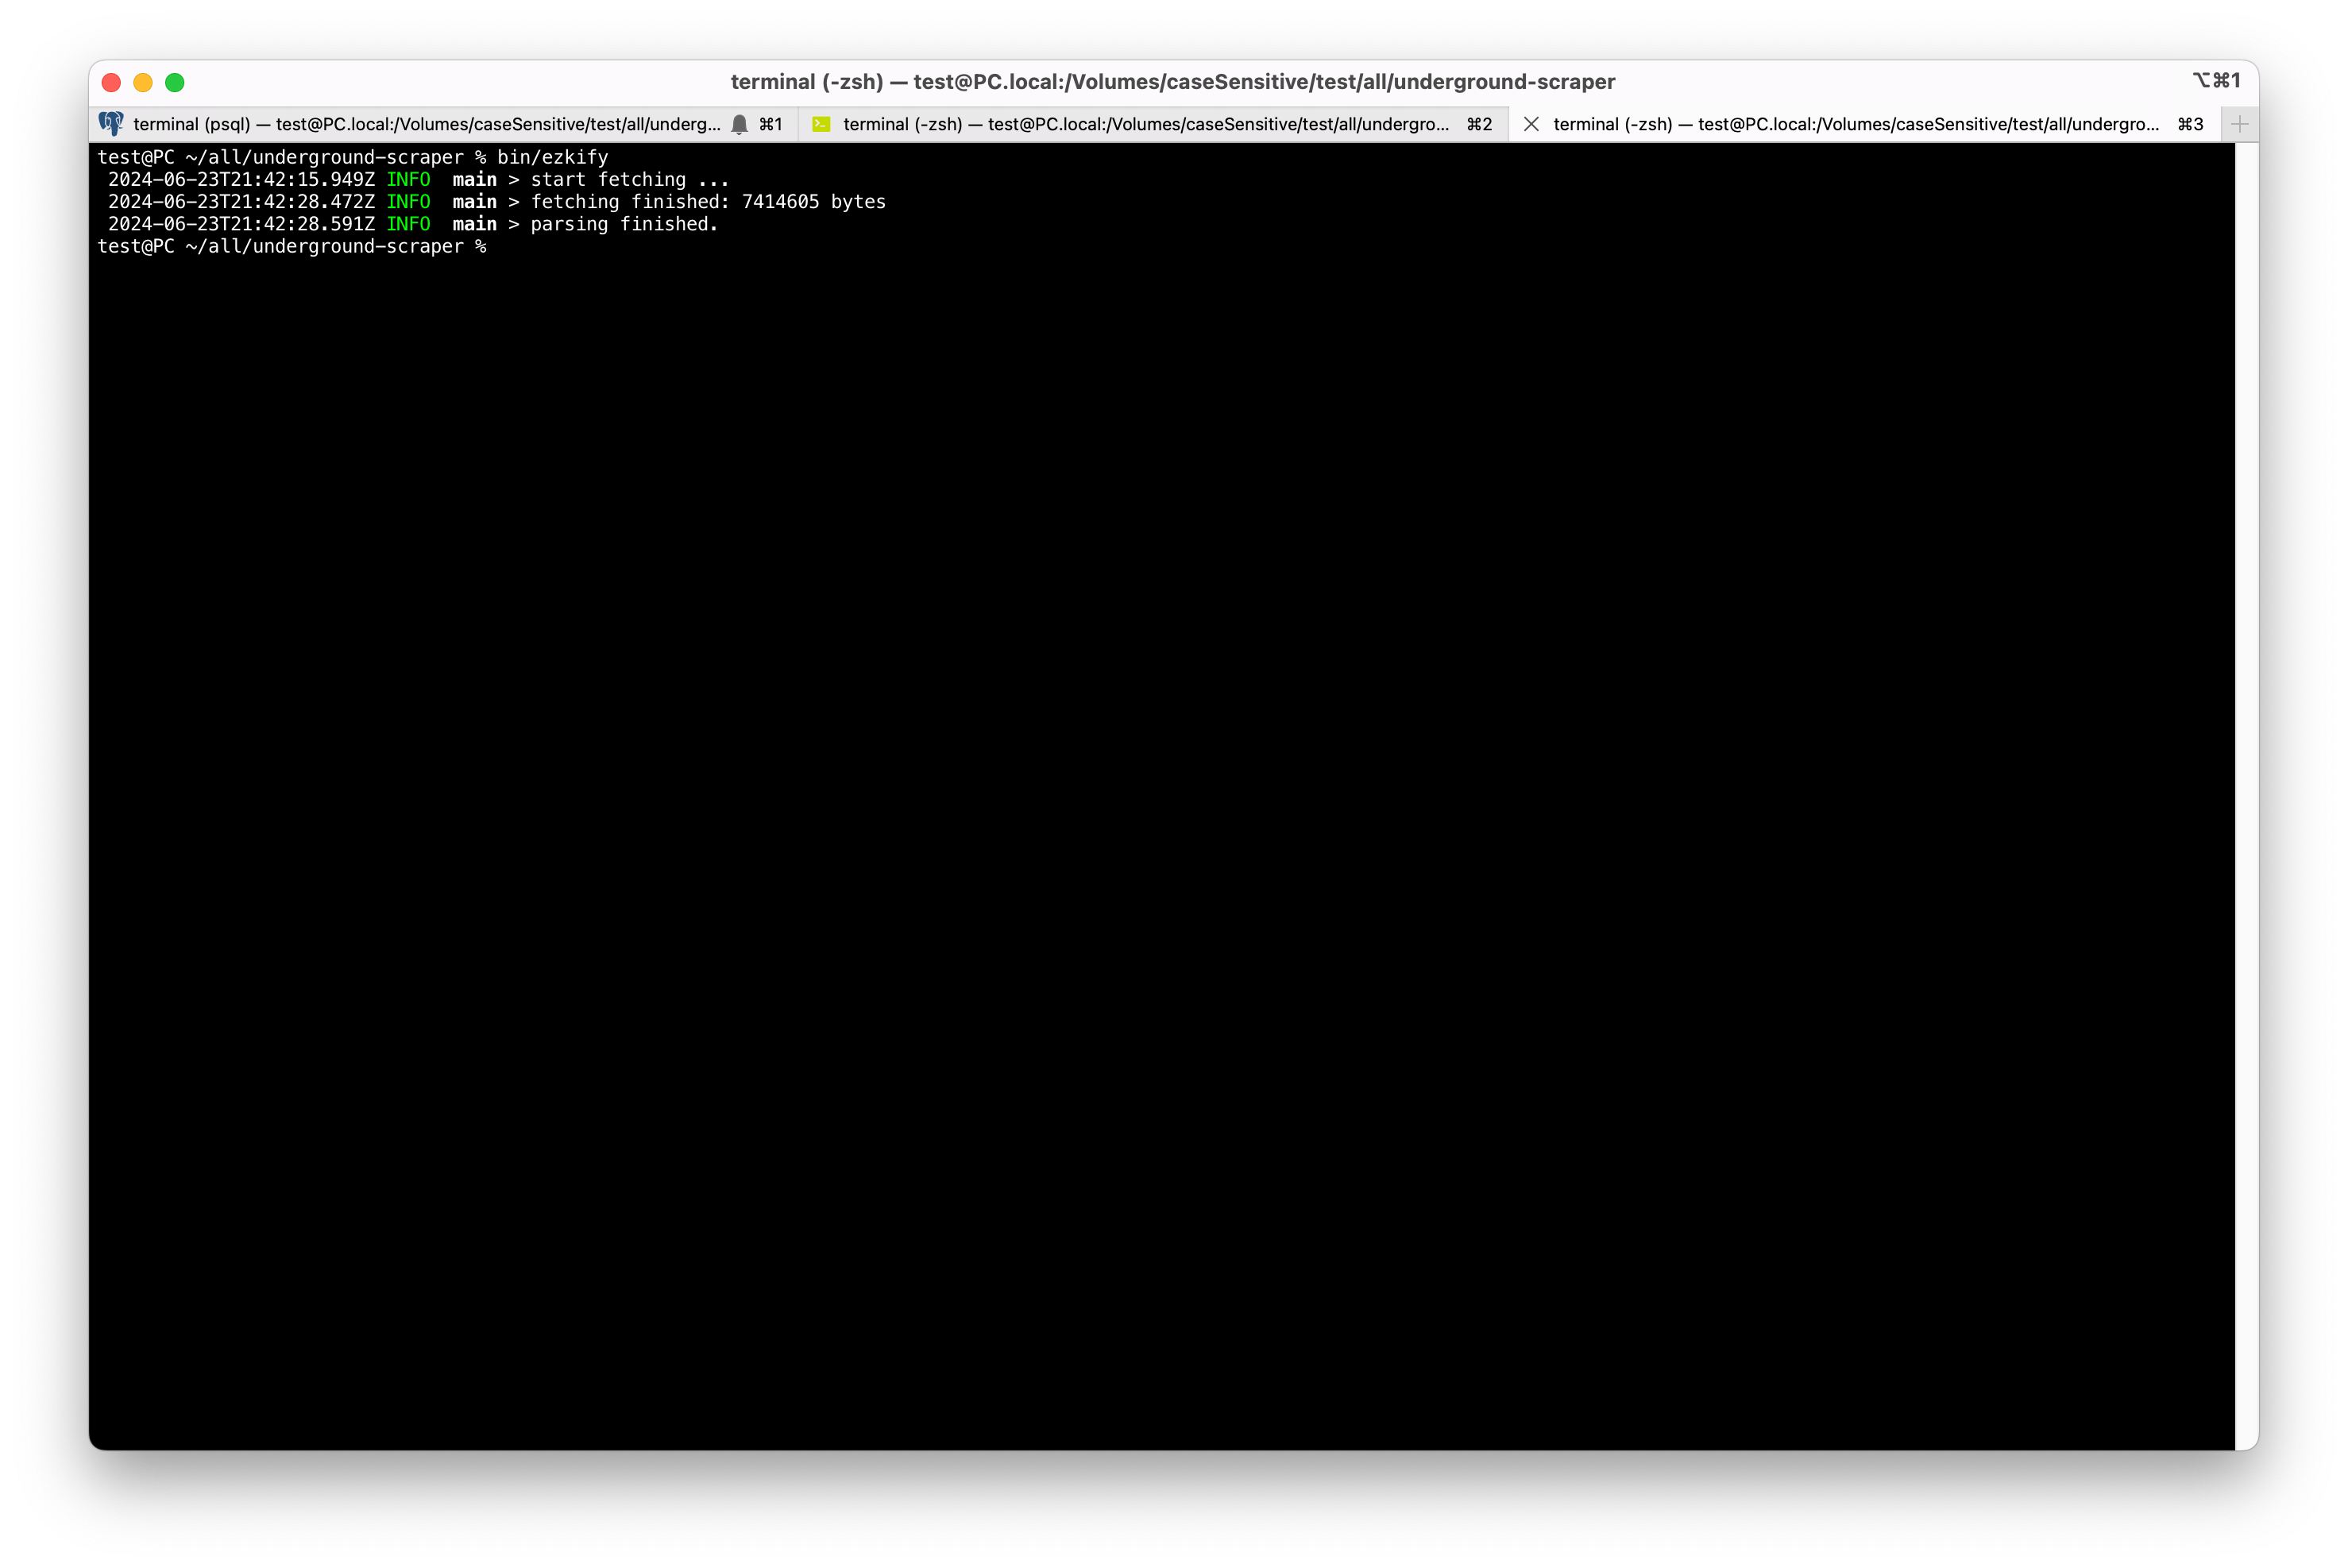
\includegraphics[scale=.17]{assets/c-e.png}
	}

	\subsubsection{BlackHatWorld}

	\frame {
		BlackHatWorld Data \pause$\begin{cases} \text{\only<4->{\color{green!80!black}}Posts List}\pause \\ \text{Content} \end{cases}$\pause

		\begin{itemize}
			\item Open a 
\includegraphics[scale=.035]{assets/chromedriver.png}ChromeDriver server at default port 9515\pause
			\item Run \texttt{./blackhatworld}\pause
			\item Solve the Cloudflare CAPTCHA \textit{if needed}
		\end{itemize}
	}

	\frame {
		BlackHatWorld Data $\begin{cases} \text{Posts List} \\ \text{\color{green!80!black}Content} \end{cases}$

		\begin{tikzpicture}
			\useasboundingbox (0, -2) rectangle (0.01, 2.5);
			\only<2->{
				\node (db) at (0, 0) {
\includegraphics[scale=.075]{assets/database.png}} node[below=20pt] {databases};
			}
			\only<3->{
				\node[draw, align=center, inner sep=2pt] (gw) at (4.5, 0) {Local Server\\(Gateway)};
				\draw[->] (gw) -- node[midway, auto, ', inner sep=1pt] {\only<8->{\color{gray}only way}} (db);
			}
			\only<4->{
				\node[draw, align=center, inner sep=2pt] (wk) at (9, 0) {Various workers\\[110pt]};
				\draw[->] (wk) -- node[midway, auto, ', inner sep=1pt] {\color{gray}HTTP} node[midway, auto, inner sep=1pt] {\color{gray}Unified} (gw);
			}
			\only<5->{
				\node[align=center] at (9, 0.8) {
\includegraphics[scale=.04]{assets/chrome.png} 
\includegraphics[scale=.05]{assets/edge.png} 
\includegraphics[scale=.014]{assets/firefox.png} 
\includegraphics[scale=.025]{assets/tor.pdf}\\[-8pt]\footnotesize Browsers, proxies};
			}
			\only<6->{
				\node[align=center] at (9, -0.7) {
\includegraphics[scale=.05]{assets/chromedriver.png} 
\includegraphics[scale=.04]{assets/ferris.png} 
\includegraphics[scale=.13]{assets/node.png} 
\includegraphics[scale=.05]{assets/python.png}\\[-8pt]\footnotesize Agents, scripts};
			}
			\only<7->{
				\node at (9, -2) {\dots\dots};
			}
			\only<9->{
				\node[draw, inner sep=2pt] (gw1) at (4.5, 2) {\texttt{./hackforums-inner}};
				\draw[->] (gw1) -- (gw);
			}
			\only<10->{
				\draw[->, fuchsia, shorten <=3pt, shorten >=3pt] (gw.north east) to[bend left=15] (wk.140);
				\draw[<-, fuchsia, shorten <=3pt, shorten >=3pt] (gw.south east) to[bend right=15] (wk.220);
				\node[fuchsia] at (6.5, 1.25) {tasks};
				\node[fuchsia] at (6.5, -1.25) {results};
			}
			\only<11->{
				\node[draw=blue, align=center, inner sep=3pt, rotate=15, fill=white, text=blue, fill opacity=.5, text opacity=1] at (7, 0) {Load balancing\\Concurrency control\\\dots\dots};
			}
			\only<12->{
				\node[draw, inner sep=2pt] (wk2) at (4, -2) {\texttt{./blackhatworld-worker config/work}};
				\draw[->] (wk2) -- (8.45, -0.6);
			}
		\end{tikzpicture}
	}
\fi
	\section{Telegram data}

	\frame {%
		\begin{columns}[c]%
			\begin{column}[c]{321pt}%
				\begin{multicols}2%
					\tableofcontents[currentsection,subsubsectionstyle=hide]%
				\end{multicols}%
			\end{column}%
		\end{columns}%
	}
\iftrue
	\subsection{Introduction}

	\frame {
		Telegram peers \pause$\begin{cases}
			\text{Users (include bots)}\pause\\
			\text{\only<6->{\color{green!80!black}}Groups}\pause\\
			\text{\only<6->{\color{green!80!black}}Channels} \\
		\end{cases}$\pause

		\begin{tikzpicture}
			\useasboundingbox (0, 0) rectangle (1pt, 1pt);
			\node[draw=red, inner sep=3pt, rotate=15, fill=white, text=red, fill opacity=.5, text opacity=1] at (4.5, 1.8) {Impossible};
		\end{tikzpicture}\pause
		\begin{itemize}
			\item Messages in Groups/Channels\pause
			\item Relations, ``Cross References'' between Groups/Channels\pause
			\item Links, Behaviors, \dots
		\end{itemize}
	}

	\subsection{Data Overview}

	\subsubsection{Results \& Attempts}

	\frame {
		\noindent\hskip-1em Dataset in 
\includegraphics[scale=.02]{assets/database.png} \pause\small$\begin{cases}
			\text{pushshift (20k+ channels, $\sim$200M messages)}\pause\\
			\text{TGDataset (121k channels, $\sim$500M messages) \only<5->{\color{gray}$\gets$ less detailed\hskip-4em\!}}\pause\\
			\text{Our own dataset (2k+ channels, $\sim$10M messages)}
		\end{cases}$\pause[6]

		\hskip5em$\color{fuchsia}\genfrac {}{}{0pt}0 \uparrow {\text{keep-up-to-date}}$\pause

		\centerline{
			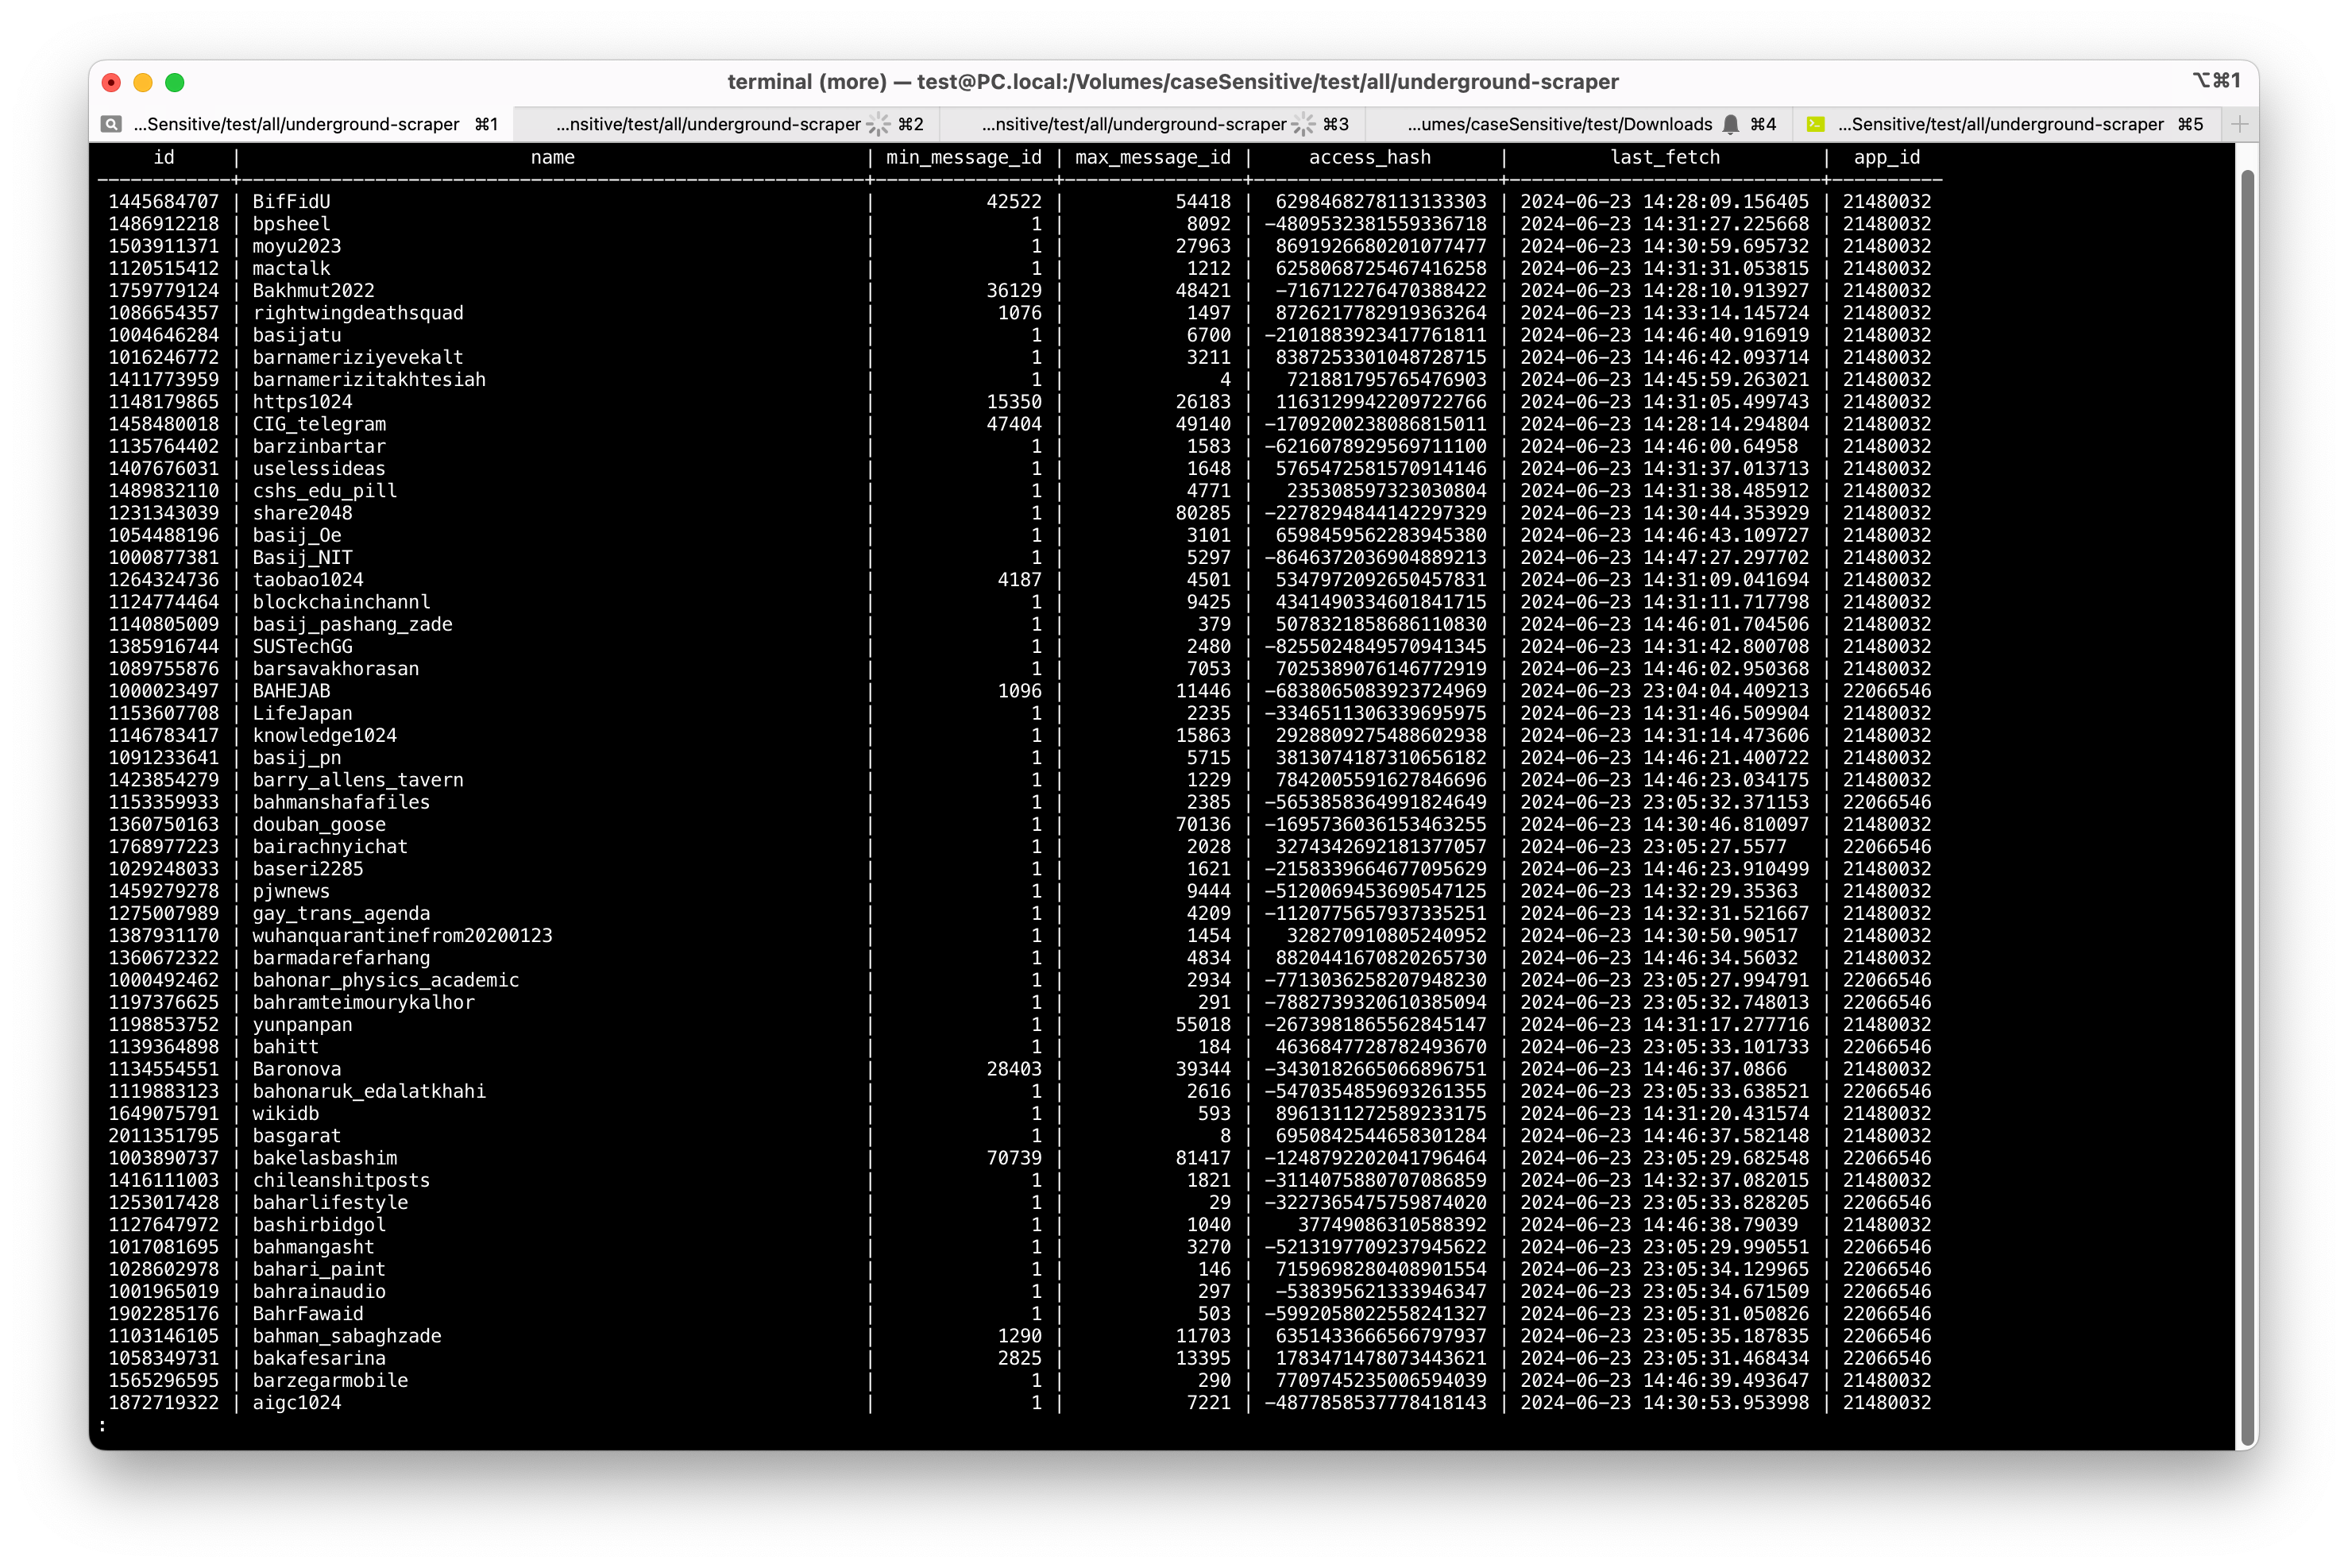
\includegraphics[scale=.125]{assets/tg1.png}\hskip-1em\pause
			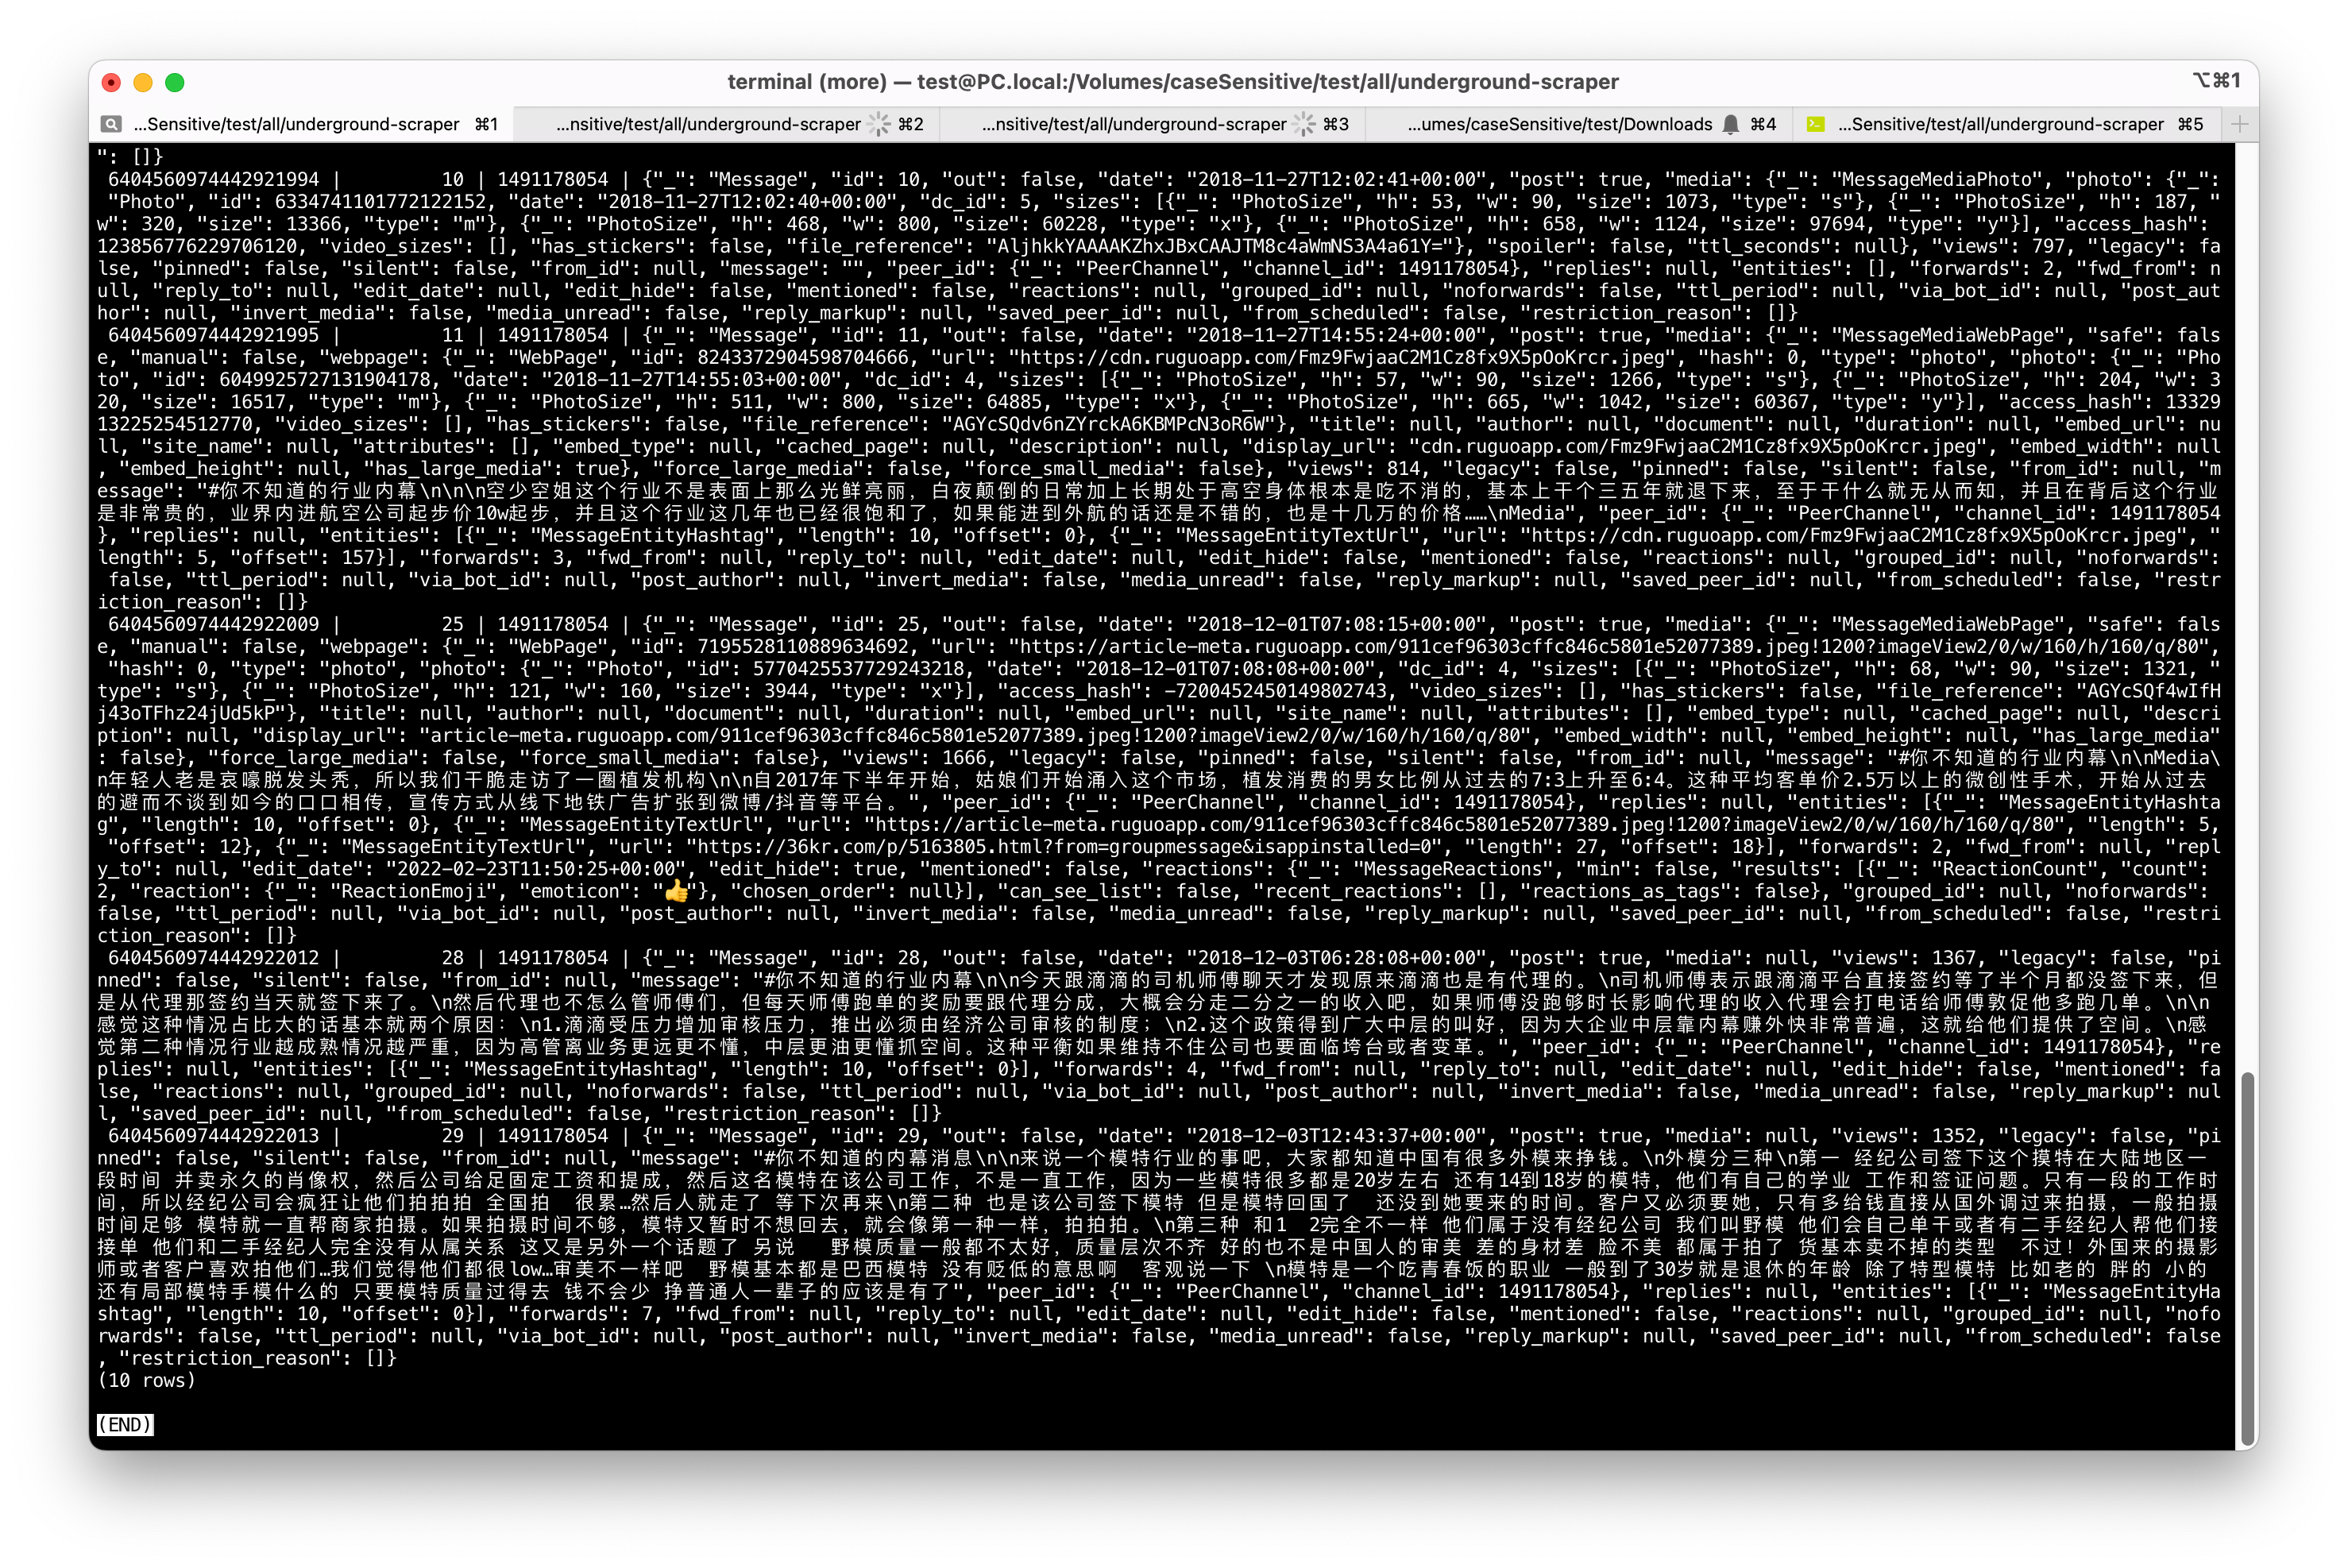
\includegraphics[scale=.125]{assets/tg2.png}
		}
	}

	\frame {
		\begin{figure}
			\centering
			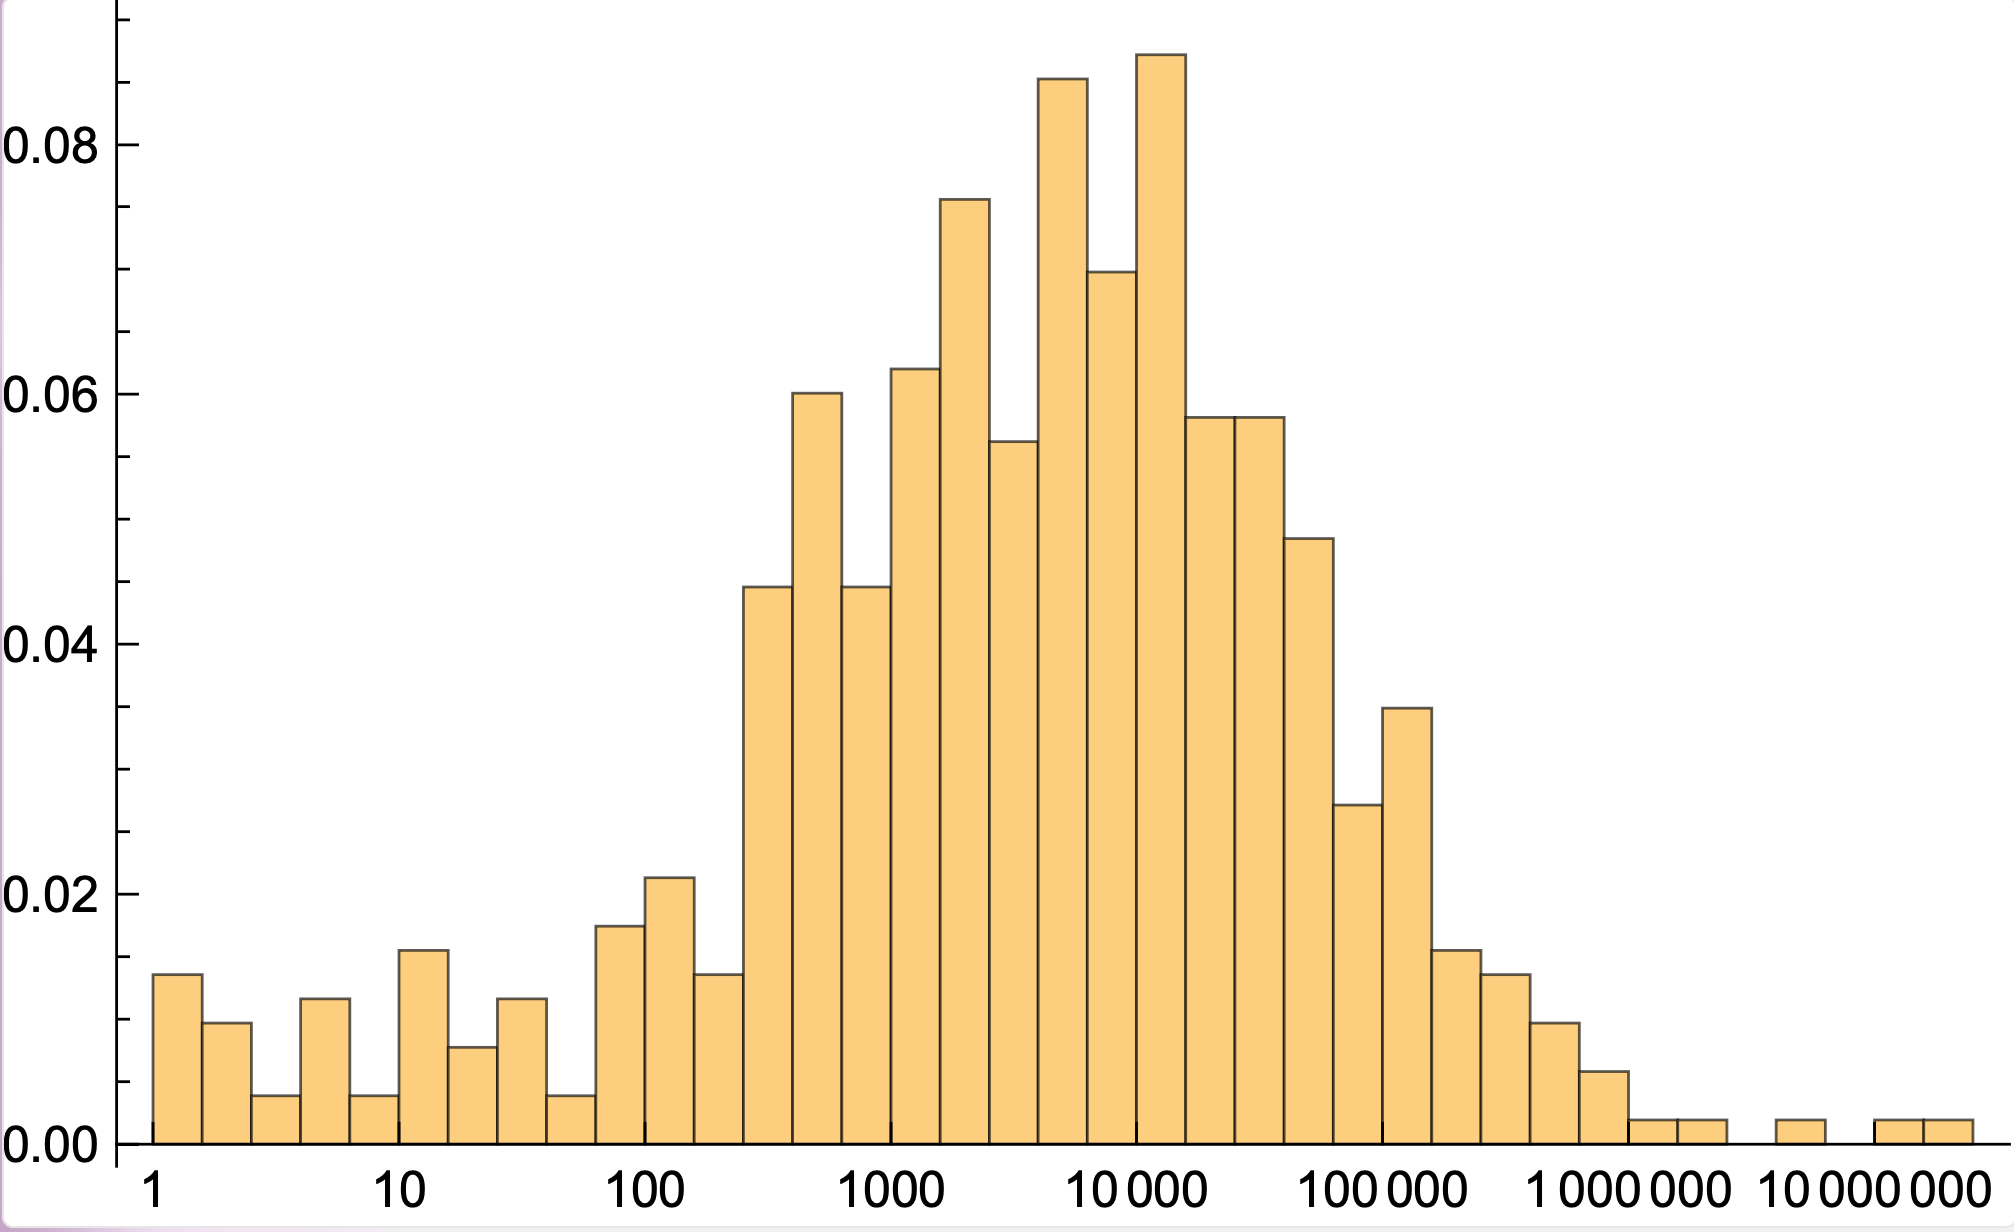
\includegraphics[scale=.14]{assets/tgh.png}
			\caption{\# (frequency) of channels with messages count in this interval}
		\end{figure}
	}

	\frame {
		\begin{figure}
			\hskip-13em
			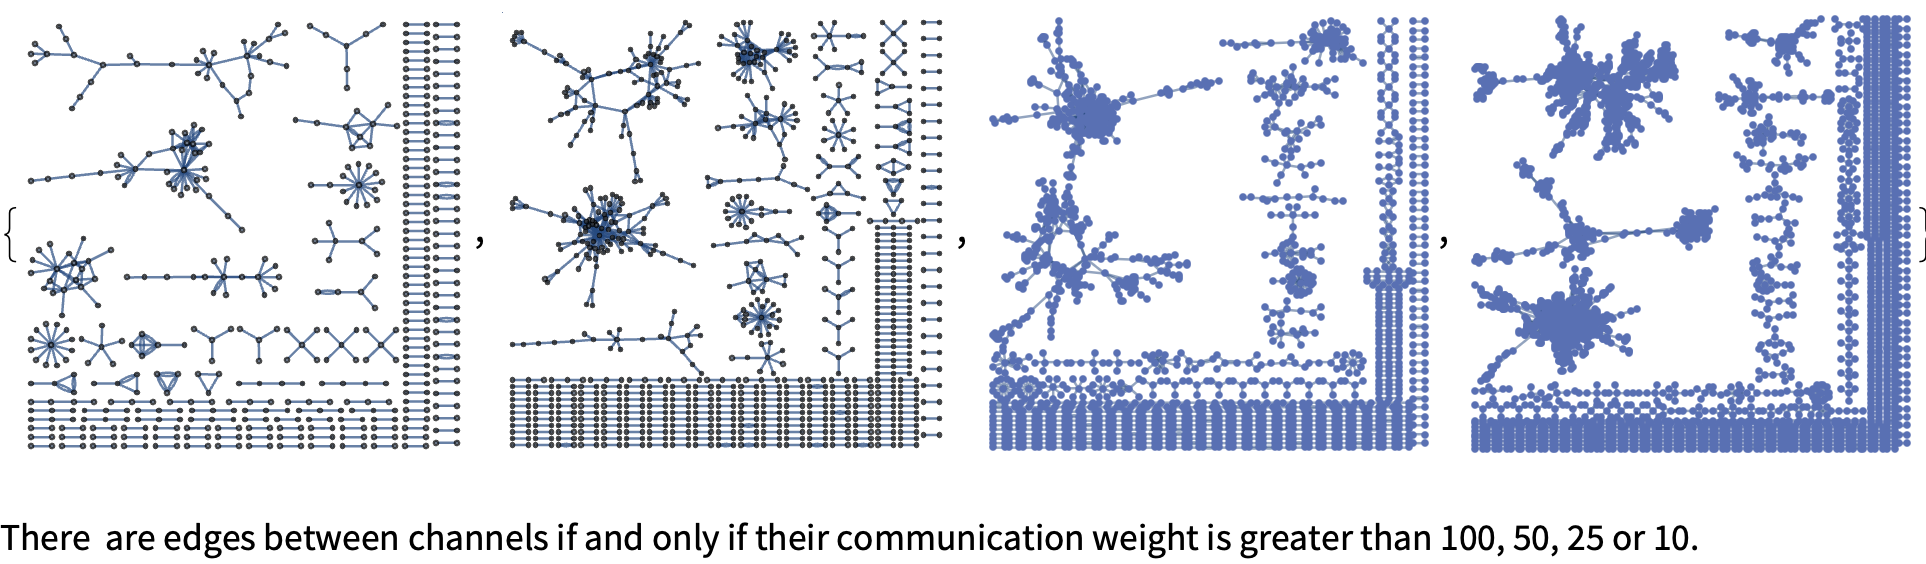
\includegraphics[scale=.18]{assets/tggr.png}
			\hskip-13em\!
			\caption{Channels/groups connection (cross-reference) graph}
		\end{figure}
	}

	\frame {
		\begin{figure}
			\centering
			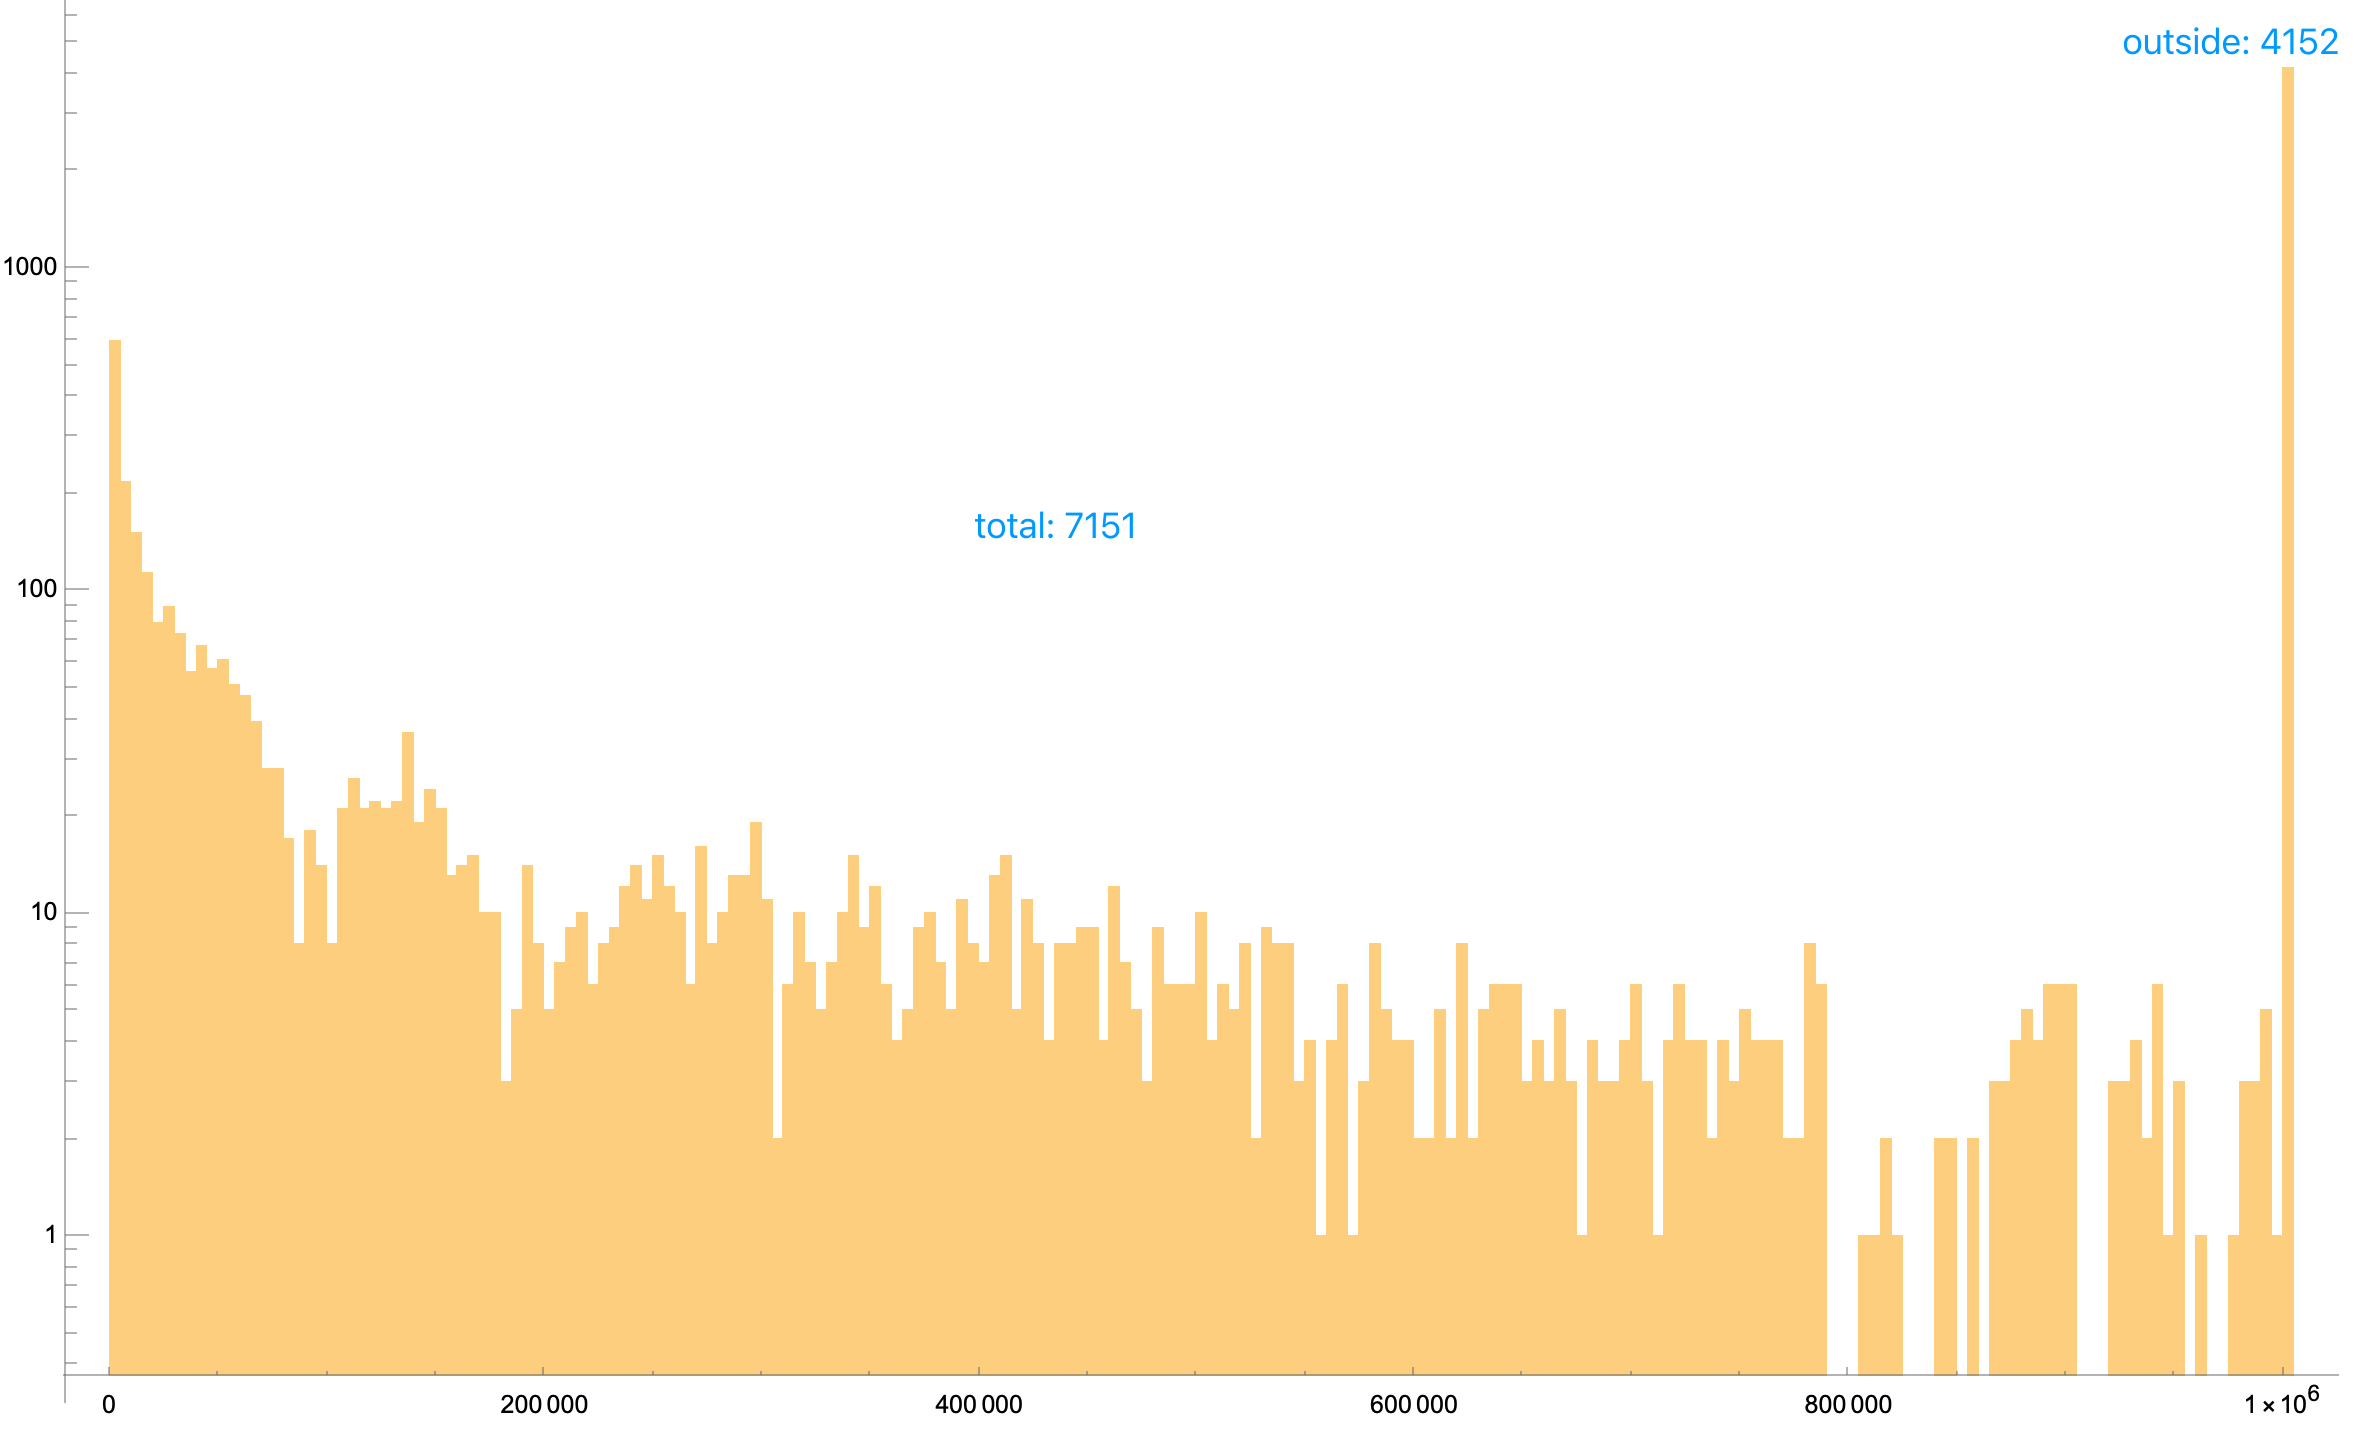
\includegraphics[scale=.12]{assets/tgdm.png}
			\caption{\# of domains appears in Bot buttons with domain ranking in this interval}
		\end{figure}
	}
\fi
	\section{Telegram scraper}

	\frame {%
		\begin{columns}[c]%
			\begin{column}[c]{321pt}%
				\begin{multicols}2%
					\tableofcontents[currentsection,subsubsectionstyle=hide]%
				\end{multicols}%
			\end{column}%
		\end{columns}%
	}
\iftrue
	\subsection{Overview}

	\frame {
		Telegram scraper:\pause
		\begin{itemize}
			\item Share workspace with previous UGM scraper\pause
			\item More flexibility, more configs/arguments/subcommand\pause
			\item More like ``using combo''
		\end{itemize}\pause

		{
			\centering
			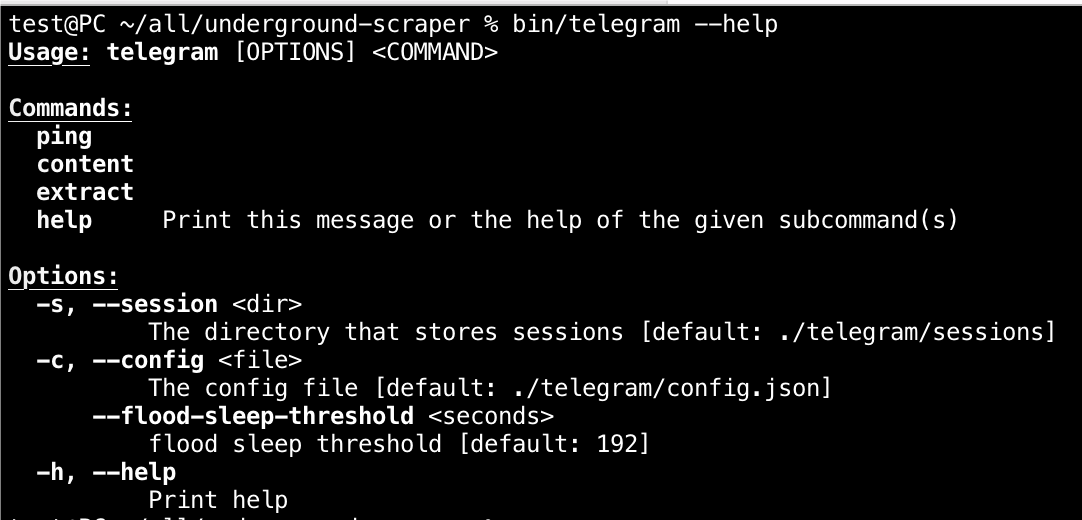
\includegraphics[scale=.2]{assets/tgclap.png}
			\par
		}
	}

	\subsection{Usage}

	\subsubsection{Rationale}

	\frame {
		\begin{tikzpicture}
			\useasboundingbox (0, 0) rectangle (1pt, 1pt);
			\node (tg) at (4.6, 2.6) {
\includegraphics[scale=.125]{assets/telegram.png}};
			\only<2->{
				\node[draw, align=left, inner sep=3pt] (idList) at (0, 0) {ID list\\[-4pt]\footnotesize Alice\\[-6pt]\footnotesize Bob\\[-8pt]\footnotesize\dots};
			}
			\only<3->{
				\node[draw, align=center, inner sep=3pt] (ah) at (3, -1) {access\\[-6pt]hashes};
				\draw[->] (idList) -- (ah);
				\draw[->] (tg) to[bend right=15] (1.5, -0.5);
			}
			\only<4->{
				\node[draw, inner sep=3pt, fuchsia] (msgs) at (6, 1) {messages};
				\draw[->, fuchsia] (idList) -- (msgs);
				\draw[->, fuchsia] (ah) -- (msgs);
				\draw[->, fuchsia] (tg) -- (4.6, .7666667);
				\draw[->, fuchsia] (4.6, .7666667) -- +(0, -.7);
			}
			\only<5->{
				\node[draw, align=left, inner sep=3pt, red] (h1) at (0.666667, 1.666667) {\footnotesize Necessary:\\[-6pt]\footnotesize(id, account)-dependent};
				\draw[->, red] (h1) -- (1.4, -0.4);
			}
			\only<6->{
				\node[draw, inner sep=2pt] (telPing) at (1.5, -2) {\texttt{\small./telegram ping -c Alice Bob ...}};
				\draw[->, dotted] (telPing) -- (1.5, -0.75);
			}
			\only<7->{
				\node[draw, inner sep=2pt, fuchsia] (telContent) at (4.6, -2.6) {\texttt{\small./telegram content}};
				\draw[->, dotted, fuchsia] (telContent) -- (4.6, 0);
			}
			\only<8-> {
				\node[draw, inner sep=3pt, blue] (urls) at (9, 1) {URLs};
				\draw[->, blue] (msgs) -- node[midway, auto, inner sep=1pt] {parser} (urls);
			}
			\only<9-> {
				\node[draw, inner sep=3pt, blue] (tiUrls) at (9, -1) {\small Telegram invitation URLs};
				\draw[->, blue] (urls) -- node[midway, auto, inner sep=1pt] {extract} (tiUrls);
			}
			\only<10->{
				\node[draw, inner sep=2pt, blue] (telex) at (8, -2) {\texttt{\small./telegram extract}};
				\draw[->, dotted, blue] (telex) -- (8, 0.9);
			}
			\only<11->{ % snowball
				\draw[->, semithick, blue] (tiUrls) -- (idList);
				\node[draw, inner sep=3pt, rotate=15, green!80!black] at (8, 2.5) {\large Snowball Sampling};
			}
		\end{tikzpicture}
	}
\fi
	\section[Workflows \& Challenges]{More on Telegram, Workflows and Challenges}

	\frame {%
		\begin{columns}[c]%
			\begin{column}[c]{321pt}%
				\begin{multicols}2%
					\tableofcontents[currentsection,subsubsectionstyle=hide]%
				\end{multicols}%
			\end{column}%
		\end{columns}%
	}
\iftrue
	\subsection{Goals \& Directions}

	\subsubsection{Roadmap}

	\frame {
		\begin{enumerate}
			\item Attempt to characterize the Telegram ecosystem
				\begin{itemize}
					\item<2-> We need a HUGE dataset
					\item<3-> Telegram has tight rate limit on username resolve
						
						\leavevmode
				\end{itemize}
			\item<6-> Dark-web markets analysis
			\item<7-> Bot behavior analysis
			\item<8-> Connection graph
			\item<9-> Data comparison with pushshift, etc.
		\end{enumerate}
		\begin{tikzpicture}
			\useasboundingbox (-1.53, -3.4) rectangle +(1pt, 1pt);
			\only<4>{\node at (3.5, 0) {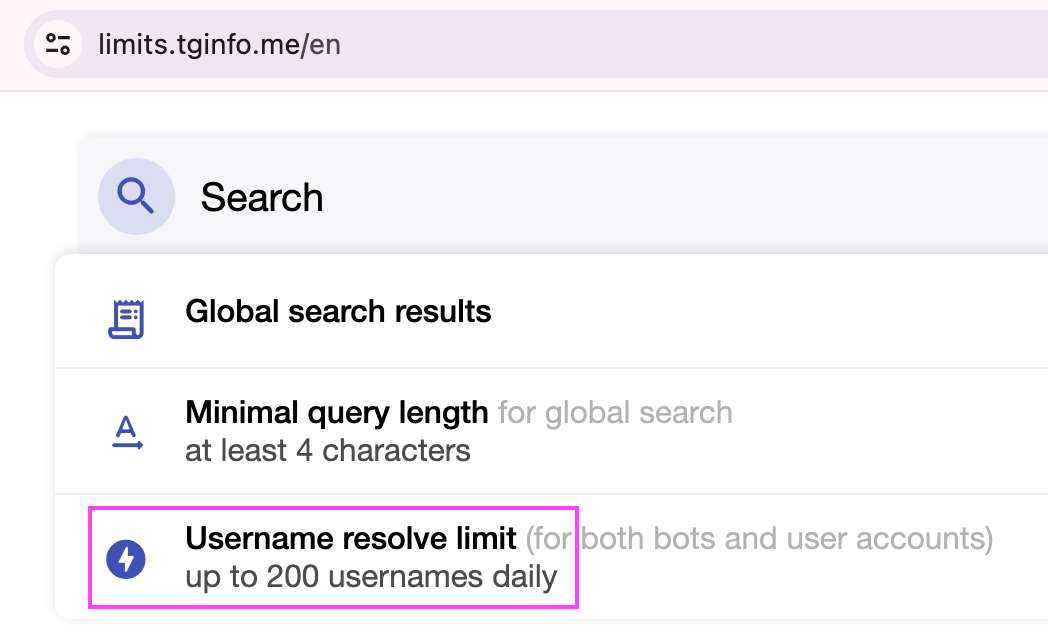
\includegraphics[scale=.4]{assets/tglimit.png}};}
			\only<5->{\node[draw=red, inner sep=3pt, rotate=15, fill=white, text=red, fill opacity=.5, text opacity=1] at (3.5, 1.25) {\large Unpractical};}
			\only<10->{
				\node[draw, inner sep=3pt, green!80!black] (present) at (0.83, 0) {Present};
				\draw[->, green!80!black] (present) -- +(0, -1);
			}
			\only<11->{
				\node[draw, align=justify, inner sep=3pt, blue] (btn) at (5.5, -1.25) {extract message, bot\\[-4pt]buttons/interactions};
				\draw[<-, blue] (btn) -- +(-2.75, 0);
			}
			\only<12->{
				\draw[->, fuchsia] (btn.north) to[bend right=15, ', "?"] (3.5, -0.5);
			}
			\only<13->{
				\node[draw, align=justify, inner sep=3pt, fuchsia] at (7.3, 0) {\small Most bots won't exposure their\\[-4pt]\small website or use other methods};
			}
			\only<14->{
				\node[draw=red, inner sep=3pt, rotate=15, fill=white, text=red, fill opacity=.5, text opacity=1] at (4.35, -0.4) {Hard};
			}
			\only<15->{
				\node[draw=properpurple, inner sep=3pt, fill=white, text=properpurple, fill opacity=.833333, text opacity=1] (topAnal) at (4.333333, -2.5) {Topic analysis};
				\node[draw, inner sep=3pt, properpurple] (urlAnal) at (7.5, -2.5) {General URL analysis};
				\draw[->, properpurple] (btn) -- (topAnal);
				\draw[->, properpurple] (btn) -- (urlAnal);
			}
			\only<16->{
				\node[draw, inner sep=3pt, properpurple] (anal1) at (5.5, -3.75) {Domain analysis};
				\node[draw, inner sep=3pt, properpurple] (anal2) at (7.5, -3.75) {\dots};
				\node[draw, inner sep=3pt, properpurple] (anal3) at (8.5, -3.75) {\dots};
				\node[draw, inner sep=3pt, properpurple] (anal4) at (9.5, -3.75) {\dots};
				\draw[->, properpurple] (urlAnal) -- (anal1);
				\draw[->, properpurple] (urlAnal) -- (anal2);
				\draw[->, properpurple] (urlAnal) -- (anal3);
				\draw[->, properpurple] (urlAnal) -- (anal4);
			}
		\end{tikzpicture}
	}

	\subsubsection{Domain analysis}

	\frame {
		\begin{tikzpicture}
			\useasboundingbox (0, 0) rectangle (1pt, 1pt);
			\node (tg) at (4.6, 2.6) {
\includegraphics[scale=.125]{assets/telegram.png}};

			\node[draw, align=left, inner sep=3pt] (idList) at (0, 0) {ID list\\[-4pt]\footnotesize Alice\\[-6pt]\footnotesize Bob\\[-8pt]\footnotesize\dots};

			\node[draw, align=center, inner sep=3pt] (ah) at (3, -1) {access\\[-6pt]hashes};
			\alt<1>{\draw[->] (idList) -- (ah);}
			{\draw[->, thick, red] (idList) -- (ah);}
			\draw[->] (tg) to[bend right=15] (1.5, -0.5); % aux

			\node[draw, inner sep=3pt, fuchsia] (msgs) at (6, 1) {messages};
			\draw[->, fuchsia] (idList) -- (msgs);
			\draw[->, fuchsia] (ah) -- (msgs);
			\draw[->, fuchsia] (tg) -- (4.6, .7666667); % aux
			\draw[->, fuchsia] (4.6, .7666667) -- +(0, -.7);

			\node[draw, inner sep=3pt, blue] (urls) at (9, 1) {URLs};
			\draw[->, blue] (msgs) -- node[midway, auto, inner sep=1pt] {parser} (urls);

			\node[draw, inner sep=3pt, blue] (tiUrls) at (9, -1) {\small Telegram invitation URLs};
			\draw[->, blue] (urls) -- node[midway, auto, inner sep=1pt] {extract} (tiUrls);

			\draw[->, semithick, blue] (tiUrls) -- (idList);
	
			\only<2->{
				\node[draw, align=left, inner sep=3pt, red] (h1) at (0.666667, 1.666667) {\footnotesize tightest pipe restriction:\\[-6pt]\footnotesize200 usernames daily};
				\draw[->, red] (h1) -- (1.4, -0.4);
			}

			\only<3-> {
				\node[draw, dashed, inner sep=3pt, properpurple] (ps) at (6.2, 2.5) {pushshift};
				\node[draw, dashed, inner sep=3pt, properpurple] (td) at (8.5, 2.5) {TGDataset};
				\draw[->, properpurple] (ps) -- (urls);
				\draw[->, properpurple] (td) -- (urls);
			}

			\only<4-> {
				\node[draw, inner sep=3pt, properpurple] (domains) at (6, -2.25) {Domains};
				\draw[->, properpurple] (urls) to[bend right=15] (domains);
			}

			\only<5-> {
				\node[draw, inner sep=3pt, properpurple] (ranking) at (3, -2.25) {Ranking};
				\draw[->, properpurple] (domains) -- (ranking);

				\node[green!80!black] (tranco) at (4.5, -3.5) {\footnotesize tranco-list.eu};
				\draw[->, properpurple] (tranco) -- (4.5, -2.25);
			}

			\only<6->{
				\node[draw, inner sep=3pt, properpurple] (analysis) at (0, -2.25) {Analysis};
				\draw[->, properpurple] (ranking) -- (analysis);
			}

			\temporal<7>{}{
				\node[draw] at (4.6, -0.4) {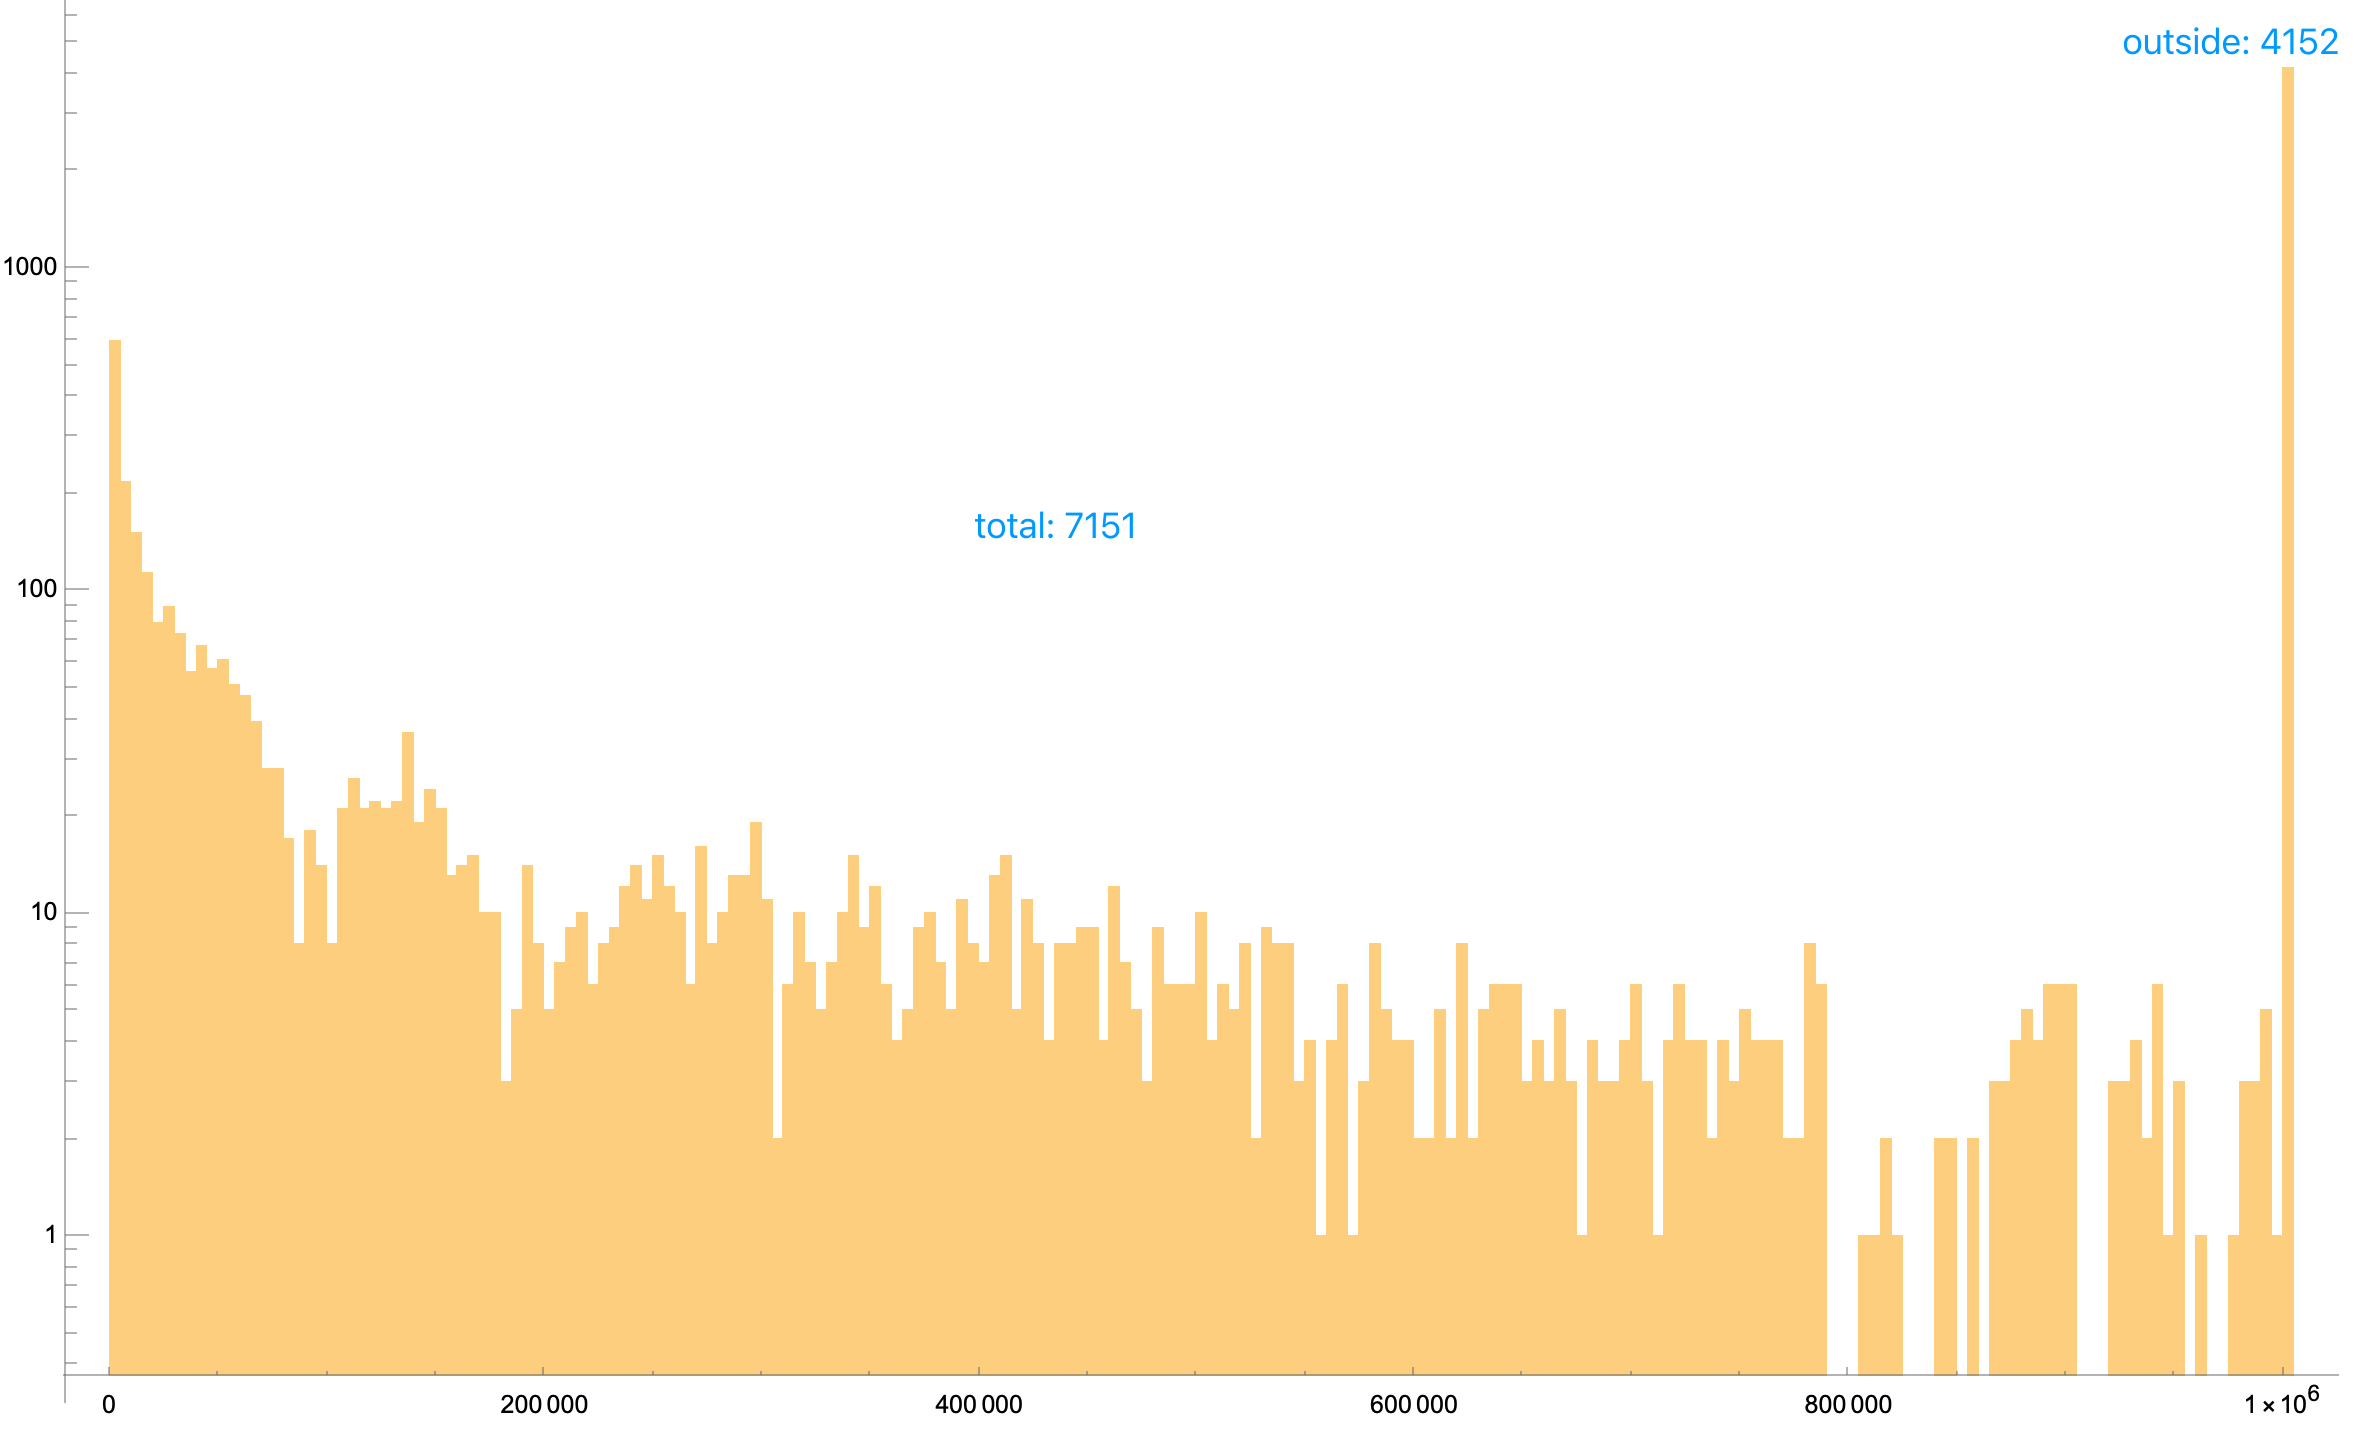
\includegraphics[scale=.12]{assets/tgdm.png}};
			}{
				\node[draw, opacity=.25] at (4.6, -0.4) {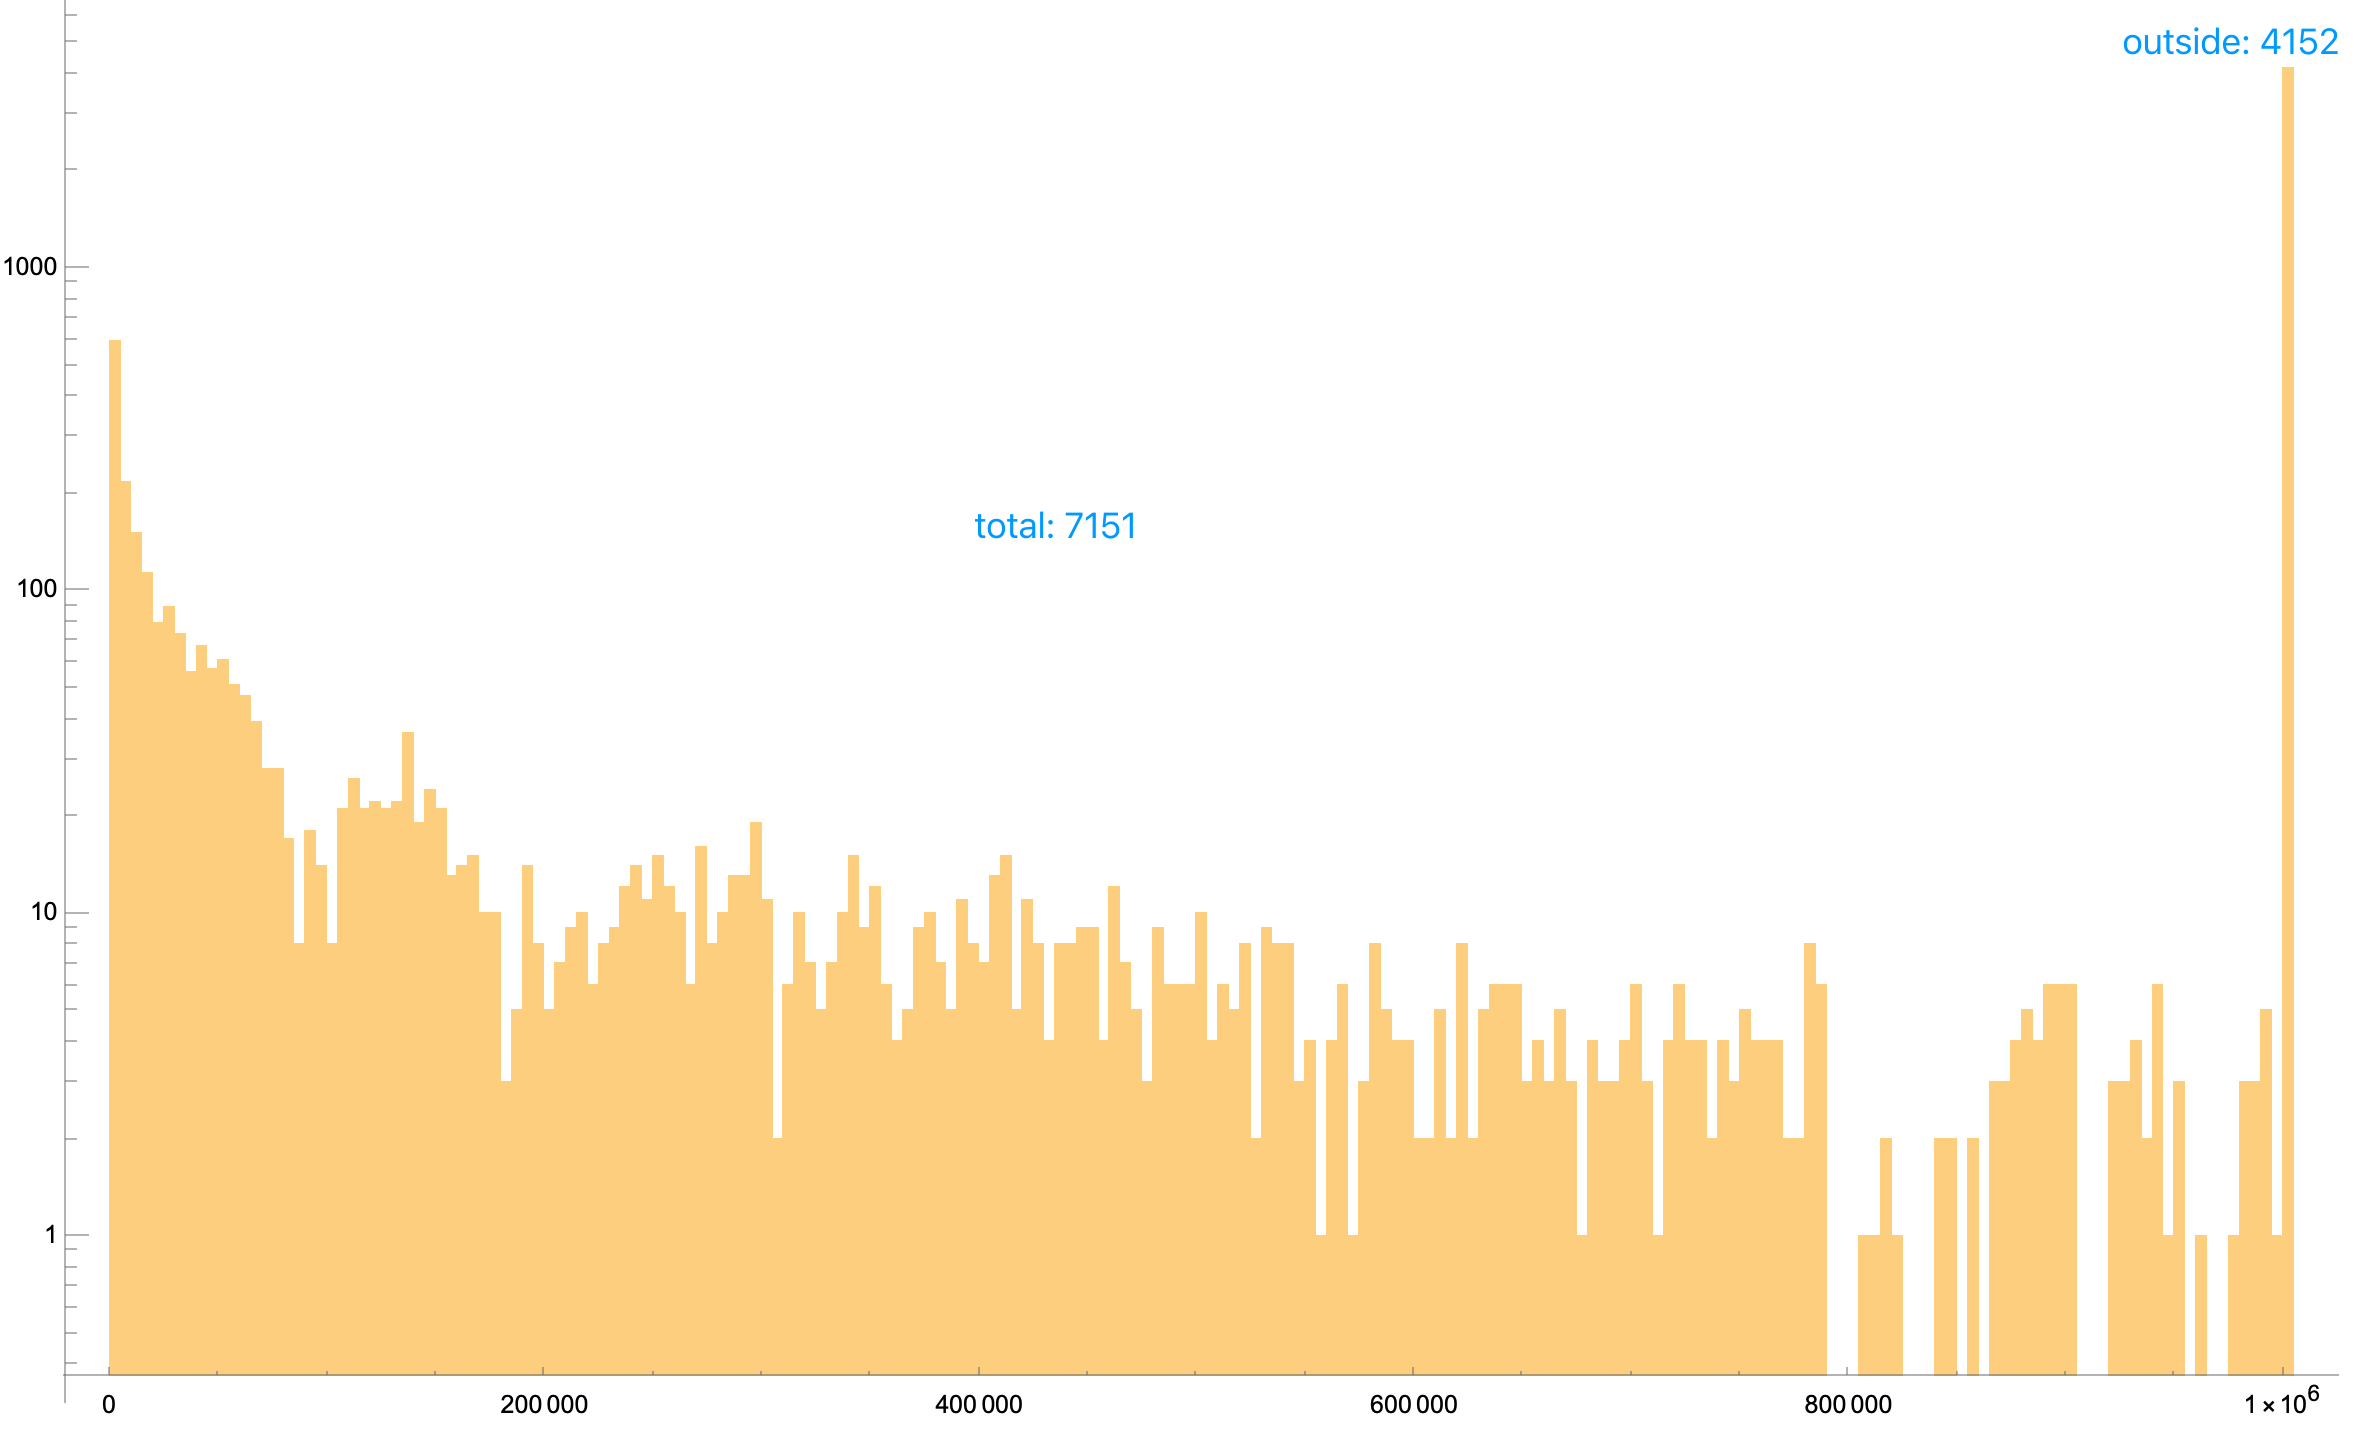
\includegraphics[scale=.12]{assets/tgdm.png}};
			}

			\only<8->{
				\draw[<->, semithick, red] (ps.225) -- (msgs.135);
				\draw[<->, semithick, red] (td.270) -- (msgs.18);
				\node[red] at (6.67, 1.75) {\scriptsize differentiate?};
			}
		\end{tikzpicture}
	}

\fi
	% \bibliographystyle{alpha}

	\setcounter{section}{-1}

	\subsection{}

	% \frame {
	% 	\scriptsize
	% 	\bibliography{slide}
	% }

	\frame {
		\centerline{Thanks for listening!}
	}
\end{document}
